\documentclass[twoside]{book}

% Packages required by doxygen
\usepackage{fixltx2e}
\usepackage{calc}
\usepackage{doxygen}
\usepackage[export]{adjustbox} % also loads graphicx
\usepackage{graphicx}
\usepackage[utf8]{inputenc}
\usepackage{makeidx}
\usepackage{multicol}
\usepackage{multirow}
\PassOptionsToPackage{warn}{textcomp}
\usepackage{textcomp}
\usepackage[nointegrals]{wasysym}
\usepackage[table]{xcolor}

% Font selection
\usepackage[T1]{fontenc}
\usepackage[scaled=.90]{helvet}
\usepackage{courier}
\usepackage{amssymb}
\usepackage{sectsty}
\renewcommand{\familydefault}{\sfdefault}
\allsectionsfont{%
  \fontseries{bc}\selectfont%
  \color{darkgray}%
}
\renewcommand{\DoxyLabelFont}{%
  \fontseries{bc}\selectfont%
  \color{darkgray}%
}
\newcommand{\+}{\discretionary{\mbox{\scriptsize$\hookleftarrow$}}{}{}}

% Page & text layout
\usepackage{geometry}
\geometry{%
  a4paper,%
  top=2.5cm,%
  bottom=2.5cm,%
  left=2.5cm,%
  right=2.5cm%
}
\tolerance=750
\hfuzz=15pt
\hbadness=750
\setlength{\emergencystretch}{15pt}
\setlength{\parindent}{0cm}
\setlength{\parskip}{3ex plus 2ex minus 2ex}
\makeatletter
\renewcommand{\paragraph}{%
  \@startsection{paragraph}{4}{0ex}{-1.0ex}{1.0ex}{%
    \normalfont\normalsize\bfseries\SS@parafont%
  }%
}
\renewcommand{\subparagraph}{%
  \@startsection{subparagraph}{5}{0ex}{-1.0ex}{1.0ex}{%
    \normalfont\normalsize\bfseries\SS@subparafont%
  }%
}
\makeatother

% Headers & footers
\usepackage{fancyhdr}
\pagestyle{fancyplain}
\fancyhead[LE]{\fancyplain{}{\bfseries\thepage}}
\fancyhead[CE]{\fancyplain{}{}}
\fancyhead[RE]{\fancyplain{}{\bfseries\leftmark}}
\fancyhead[LO]{\fancyplain{}{\bfseries\rightmark}}
\fancyhead[CO]{\fancyplain{}{}}
\fancyhead[RO]{\fancyplain{}{\bfseries\thepage}}
\fancyfoot[LE]{\fancyplain{}{}}
\fancyfoot[CE]{\fancyplain{}{}}
\fancyfoot[RE]{\fancyplain{}{\bfseries\scriptsize Generated by Doxygen }}
\fancyfoot[LO]{\fancyplain{}{\bfseries\scriptsize Generated by Doxygen }}
\fancyfoot[CO]{\fancyplain{}{}}
\fancyfoot[RO]{\fancyplain{}{}}
\renewcommand{\footrulewidth}{0.4pt}
\renewcommand{\chaptermark}[1]{%
  \markboth{#1}{}%
}
\renewcommand{\sectionmark}[1]{%
  \markright{\thesection\ #1}%
}

% Indices & bibliography
\usepackage{natbib}
\usepackage[titles]{tocloft}
\setcounter{tocdepth}{3}
\setcounter{secnumdepth}{5}
\makeindex

% Hyperlinks (required, but should be loaded last)
\usepackage{ifpdf}
\ifpdf
  \usepackage[pdftex,pagebackref=true]{hyperref}
\else
  \usepackage[ps2pdf,pagebackref=true]{hyperref}
\fi
\hypersetup{%
  colorlinks=true,%
  linkcolor=blue,%
  citecolor=blue,%
  unicode%
}

% Custom commands
\newcommand{\clearemptydoublepage}{%
  \newpage{\pagestyle{empty}\cleardoublepage}%
}

\usepackage{caption}
\captionsetup{labelsep=space,justification=centering,font={bf},singlelinecheck=off,skip=4pt,position=top}

%===== C O N T E N T S =====

\begin{document}

% Titlepage & ToC
\hypersetup{pageanchor=false,
             bookmarksnumbered=true,
             pdfencoding=unicode
            }
\pagenumbering{alph}
\begin{titlepage}
\vspace*{7cm}
\begin{center}%
{\Large My Project }\\
\vspace*{1cm}
{\large Generated by Doxygen 1.8.13}\\
\end{center}
\end{titlepage}
\clearemptydoublepage
\pagenumbering{roman}
\tableofcontents
\clearemptydoublepage
\pagenumbering{arabic}
\hypersetup{pageanchor=true}

%--- Begin generated contents ---
\chapter{Hierarchical Index}
\doxysection{Class Hierarchy}
This inheritance list is sorted roughly, but not completely, alphabetically\+:\begin{DoxyCompactList}
\item \contentsline{section}{BC}{\pageref{classBC}}{}
\item \contentsline{section}{Bulk}{\pageref{classBulk}}{}
\item \contentsline{section}{Bulk\+Datum}{\pageref{classBulkDatum}}{}
\item \contentsline{section}{F\+EM}{\pageref{classFEM}}{}
\item grammar\begin{DoxyCompactList}
\item \contentsline{section}{LifeV\+::Parser\+Spirit\+Grammar$<$ Iterator\+Type, Results\+Type $>$}{\pageref{classLifeV_1_1ParserSpiritGrammar}}{}
\item \contentsline{section}{LifeV\+::Parser\+Spirit\+Grammar$<$ string\+Iterator\+\_\+\+Type $>$}{\pageref{classLifeV_1_1ParserSpiritGrammar}}{}
\end{DoxyCompactList}
\item \contentsline{section}{Linear\+System}{\pageref{classLinearSystem}}{}
\item \contentsline{section}{LifeV\+::Parser}{\pageref{classLifeV_1_1Parser}}{}
\item \contentsline{section}{Problem}{\pageref{classProblem}}{}
\begin{DoxyCompactList}
\item \contentsline{section}{Basic\+Method}{\pageref{classBasicMethod}}{}
\begin{DoxyCompactList}
\item \contentsline{section}{Laplacian\+Basic}{\pageref{classLaplacianBasic}}{}
\item \contentsline{section}{Linear\+Elasticity\+Basic}{\pageref{classLinearElasticityBasic}}{}
\end{DoxyCompactList}
\item \contentsline{section}{Symmetric\+Method}{\pageref{classSymmetricMethod}}{}
\begin{DoxyCompactList}
\item \contentsline{section}{Laplacian\+Symmetric}{\pageref{classLaplacianSymmetric}}{}
\item \contentsline{section}{Linear\+Elasticity\+Symmetric}{\pageref{classLinearElasticitySymmetric}}{}
\end{DoxyCompactList}
\end{DoxyCompactList}
\end{DoxyCompactList}

\chapter{Class Index}
\doxysection{Class List}
Here are the classes, structs, unions and interfaces with brief descriptions\+:\begin{DoxyCompactList}
\item\contentsline{section}{\mbox{\hyperlink{classBasicMethod}{Basic\+Method}} }{\pageref{classBasicMethod}}{}
\item\contentsline{section}{\mbox{\hyperlink{classBC}{BC}} }{\pageref{classBC}}{}
\item\contentsline{section}{\mbox{\hyperlink{classBulk}{Bulk}} }{\pageref{classBulk}}{}
\item\contentsline{section}{\mbox{\hyperlink{classBulkDatum}{Bulk\+Datum}} }{\pageref{classBulkDatum}}{}
\item\contentsline{section}{\mbox{\hyperlink{classFEM}{F\+EM}} }{\pageref{classFEM}}{}
\item\contentsline{section}{\mbox{\hyperlink{classLaplacianBasic}{Laplacian\+Basic}} }{\pageref{classLaplacianBasic}}{}
\item\contentsline{section}{\mbox{\hyperlink{classLaplacianSymmetric}{Laplacian\+Symmetric}} }{\pageref{classLaplacianSymmetric}}{}
\item\contentsline{section}{\mbox{\hyperlink{classLinearElasticityBasic}{Linear\+Elasticity\+Basic}} }{\pageref{classLinearElasticityBasic}}{}
\item\contentsline{section}{\mbox{\hyperlink{classLinearElasticitySymmetric}{Linear\+Elasticity\+Symmetric}} }{\pageref{classLinearElasticitySymmetric}}{}
\item\contentsline{section}{\mbox{\hyperlink{classLinearSystem}{Linear\+System}} }{\pageref{classLinearSystem}}{}
\item\contentsline{section}{\mbox{\hyperlink{classLifeV_1_1Parser}{Life\+V\+::\+Parser}} \\*\mbox{\hyperlink{classLifeV_1_1Parser}{Parser}} -\/ A string parser for algebraic expressions }{\pageref{classLifeV_1_1Parser}}{}
\item\contentsline{section}{\mbox{\hyperlink{classLifeV_1_1ParserSpiritGrammar}{Life\+V\+::\+Parser\+Spirit\+Grammar$<$ Iterator\+Type, Results\+Type $>$}} \\*\mbox{\hyperlink{classLifeV_1_1ParserSpiritGrammar}{Parser\+Spirit\+Grammar}} -\/ A string parser grammar based on {\ttfamily boost\+::spirit\+::qi} }{\pageref{classLifeV_1_1ParserSpiritGrammar}}{}
\item\contentsline{section}{\mbox{\hyperlink{classProblem}{Problem}} }{\pageref{classProblem}}{}
\item\contentsline{section}{\mbox{\hyperlink{classSymmetricMethod}{Symmetric\+Method}} }{\pageref{classSymmetricMethod}}{}
\end{DoxyCompactList}

\chapter{File Index}
\section{File List}
Here is a list of all documented files with brief descriptions\+:\begin{DoxyCompactList}
\item\contentsline{section}{include/{\bfseries B\+C.\+h} }{\pageref{BC_8h}}{}
\item\contentsline{section}{include/{\bfseries Bulk.\+h} }{\pageref{Bulk_8h}}{}
\item\contentsline{section}{include/\hyperlink{BulkDatum_8h}{Bulk\+Datum.\+h} }{\pageref{BulkDatum_8h}}{}
\item\contentsline{section}{include/{\bfseries Core.\+h} }{\pageref{Core_8h}}{}
\item\contentsline{section}{include/{\bfseries F\+E\+M.\+h} }{\pageref{FEM_8h}}{}
\item\contentsline{section}{include/{\bfseries Laplacian\+Pb.\+h} }{\pageref{LaplacianPb_8h}}{}
\item\contentsline{section}{include/{\bfseries Linear\+Elasticity\+Pb.\+h} }{\pageref{LinearElasticityPb_8h}}{}
\item\contentsline{section}{include/{\bfseries Linear\+System.\+h} }{\pageref{LinearSystem_8h}}{}
\item\contentsline{section}{include/{\bfseries Operators.\+h} }{\pageref{Operators_8h}}{}
\item\contentsline{section}{include/{\bfseries Operators\+B\+D.\+h} }{\pageref{OperatorsBD_8h}}{}
\item\contentsline{section}{include/{\bfseries Operators\+Bulk.\+h} }{\pageref{OperatorsBulk_8h}}{}
\item\contentsline{section}{include/\hyperlink{Parser_8h}{Parser.\+h} \\*File containing the Parser interface }{\pageref{Parser_8h}}{}
\item\contentsline{section}{include/\hyperlink{ParserDefinitions_8h}{Parser\+Definitions.\+h} \\*File containing the Parser definitions }{\pageref{ParserDefinitions_8h}}{}
\item\contentsline{section}{include/\hyperlink{ParserSpiritGrammar_8h}{Parser\+Spirit\+Grammar.\+h} \\*File containing the Parser grammar }{\pageref{ParserSpiritGrammar_8h}}{}
\item\contentsline{section}{include/{\bfseries Problem.\+h} }{\pageref{Problem_8h}}{}
\item\contentsline{section}{include/\hyperlink{StringUtility_8h}{String\+Utility.\+h} \\*Std\+::string utilities }{\pageref{StringUtility_8h}}{}
\item\contentsline{section}{include/{\bfseries Useful\+Functions.\+h} }{\pageref{UsefulFunctions_8h}}{}
\end{DoxyCompactList}

\chapter{Class Documentation}
\hypertarget{classBC}{}\section{BC Class Reference}
\label{classBC}\index{BC@{BC}}
\subsection*{Public Member Functions}
\begin{DoxyCompactItemize}
\item 
\mbox{\Hypertarget{classBC_a649dc10a83ab3fa696a17b28c2c12623}\label{classBC_a649dc10a83ab3fa696a17b28c2c12623}} 
{\bfseries BC} (const Get\+Pot \&data\+File, const std\+::string \&problem, const std\+::string \&section)
\item 
\mbox{\Hypertarget{classBC_a27a056716478adebe4e35c9bac270f92}\label{classBC_a27a056716478adebe4e35c9bac270f92}} 
void {\bfseries set\+Boundaries} (getfem\+::mesh \&mesh\+Ref)
\item 
\mbox{\Hypertarget{classBC_a047d12487d15077f4f309f346ae30c64}\label{classBC_a047d12487d15077f4f309f346ae30c64}} 
std\+::vector$<$ size\+\_\+type $>$ {\bfseries get\+Neum\+BD} () const
\item 
\mbox{\Hypertarget{classBC_a48fdb2ed8fd73b082636af6e835c4fa7}\label{classBC_a48fdb2ed8fd73b082636af6e835c4fa7}} 
std\+::vector$<$ size\+\_\+type $>$ {\bfseries get\+Diri\+BD} () const
\item 
\mbox{\Hypertarget{classBC_af50f436f390056c8a4c062c5376db48b}\label{classBC_af50f436f390056c8a4c062c5376db48b}} 
scalar\+\_\+type {\bfseries B\+C\+Neum} (const base\+\_\+node \&x, const size\+\_\+type what, const size\+\_\+type \&flag)
\item 
\mbox{\Hypertarget{classBC_a50c34e6e8a954d6625ffd4b27d58e554}\label{classBC_a50c34e6e8a954d6625ffd4b27d58e554}} 
scalar\+\_\+type {\bfseries B\+C\+Diri} (const base\+\_\+node \&x, const size\+\_\+type what, const size\+\_\+type \&flag)
\end{DoxyCompactItemize}


The documentation for this class was generated from the following file\+:\begin{DoxyCompactItemize}
\item 
include/B\+C.\+h\end{DoxyCompactItemize}

\hypertarget{classBulk}{}\section{Bulk Class Reference}
\label{classBulk}\index{Bulk@{Bulk}}
\subsection*{Public Member Functions}
\begin{DoxyCompactItemize}
\item 
\mbox{\Hypertarget{classBulk_a52311ede3fef330f838101a940549cea}\label{classBulk_a52311ede3fef330f838101a940549cea}} 
{\bfseries Bulk} (const Get\+Pot \&data\+File, const std\+::string \&section=\char`\"{}bulk\+Data/\char`\"{}, const std\+::string \&section\+Domain=\char`\"{}domain/\char`\"{}, const std\+::string \&section\+Problem=\char`\"{}nothing\char`\"{}, const std\+::string \&domain\+Number=\char`\"{}nothing\char`\"{})
\item 
\mbox{\Hypertarget{classBulk_ab54e35b72fef70d7842a2e001a63b489}\label{classBulk_ab54e35b72fef70d7842a2e001a63b489}} 
void {\bfseries export\+Mesh} (std\+::string const nomefile) const
\item 
\mbox{\Hypertarget{classBulk_a720b2466afc7935d8faa7df5b4fa86d2}\label{classBulk_a720b2466afc7935d8faa7df5b4fa86d2}} 
getfem\+::mesh \& {\bfseries get\+Mesh\+Ref} ()
\item 
\mbox{\Hypertarget{classBulk_abb9ee278cc489a52a07b802efdf7299f}\label{classBulk_abb9ee278cc489a52a07b802efdf7299f}} 
getfem\+::mesh {\bfseries get\+Mesh} () const
\item 
\mbox{\Hypertarget{classBulk_a9c779bc19573844daa5762ddf804e06b}\label{classBulk_a9c779bc19573844daa5762ddf804e06b}} 
scalar\+\_\+type {\bfseries Lx} () const
\item 
\mbox{\Hypertarget{classBulk_a89999939678abaab470a80fba071b919}\label{classBulk_a89999939678abaab470a80fba071b919}} 
scalar\+\_\+type {\bfseries Ly} () const
\item 
\mbox{\Hypertarget{classBulk_a559078ee075212bb5e6d84d575cefd46}\label{classBulk_a559078ee075212bb5e6d84d575cefd46}} 
scalar\+\_\+type {\bfseries n\+SubX} () const
\item 
\mbox{\Hypertarget{classBulk_adfe15f93582879cdf187c8ce56ccd758}\label{classBulk_adfe15f93582879cdf187c8ce56ccd758}} 
scalar\+\_\+type {\bfseries n\+SubY} () const
\end{DoxyCompactItemize}


The documentation for this class was generated from the following file\+:\begin{DoxyCompactItemize}
\item 
include/Bulk.\+h\end{DoxyCompactItemize}

\hypertarget{classBulkDatum}{}\section{Bulk\+Datum Class Reference}
\label{classBulkDatum}\index{Bulk\+Datum@{Bulk\+Datum}}
\subsection*{Public Member Functions}
\begin{DoxyCompactItemize}
\item 
\mbox{\Hypertarget{classBulkDatum_acad0930f8dadb2ca18d1c947c5f1b5d2}\label{classBulkDatum_acad0930f8dadb2ca18d1c947c5f1b5d2}} 
{\bfseries Bulk\+Datum} (const Get\+Pot \&data\+File, const std\+::string \&section, const std\+::string \&section\+Problem, const std\+::string \&domain\+Number, const std\+::string \&datum)
\item 
scalar\+\_\+type \hyperlink{classBulkDatum_ac10d12a1f4a6bd00f7978d085d417389}{get\+Value} (const base\+\_\+node \&x, const size\+\_\+type what)
\begin{DoxyCompactList}\small\item\em method to evaluate the string. \end{DoxyCompactList}\end{DoxyCompactItemize}


\subsection{Member Function Documentation}
\mbox{\Hypertarget{classBulkDatum_ac10d12a1f4a6bd00f7978d085d417389}\label{classBulkDatum_ac10d12a1f4a6bd00f7978d085d417389}} 
\index{Bulk\+Datum@{Bulk\+Datum}!get\+Value@{get\+Value}}
\index{get\+Value@{get\+Value}!Bulk\+Datum@{Bulk\+Datum}}
\subsubsection{\texorpdfstring{get\+Value()}{getValue()}}
{\footnotesize\ttfamily scalar\+\_\+type Bulk\+Datum\+::get\+Value (\begin{DoxyParamCaption}\item[{const base\+\_\+node \&}]{x,  }\item[{const size\+\_\+type}]{what }\end{DoxyParamCaption})}



method to evaluate the string. 

This method takes two input parameters and returns a scalar value.


\begin{DoxyParams}{Parameters}
{\em x} & coordinates of the point where we want to evaluate the function. \\
\hline
{\em what} & index 0 if the datum is a scalar or if we want the first component of the vector; index 1 if we want to evaluate the second component. \\
\hline
\end{DoxyParams}


The documentation for this class was generated from the following file\+:\begin{DoxyCompactItemize}
\item 
include/\hyperlink{BulkDatum_8h}{Bulk\+Datum.\+h}\end{DoxyCompactItemize}

\hypertarget{classFEM}{}\doxysection{F\+EM Class Reference}
\label{classFEM}\index{FEM@{FEM}}
\doxysubsection*{Public Member Functions}
\begin{DoxyCompactItemize}
\item 
\mbox{\hyperlink{classFEM_ab722fcdf05eac04282372946c105cf15}{F\+EM}} (const getfem\+::mesh \&mesh, const Get\+Pot \&data\+File, const std\+::string \&problem, const std\+::string \&variable, const std\+::string \&section=\char`\"{}bulk\+Data/\char`\"{}, const size\+\_\+type qdim=1)
\item 
\mbox{\hyperlink{classFEM_ac2a4a8bc61409257f613bea6cc536e9f}{F\+EM}} (const getfem\+::mesh \&mesh, const std\+::string fem\+Type, const size\+\_\+type space\+Dim)
\item 
\mbox{\Hypertarget{classFEM_aac29709ad2ddb308ae62740bfcd37e00}\label{classFEM_aac29709ad2ddb308ae62740bfcd37e00}} 
size\+\_\+type {\bfseries nb\+\_\+dof} () const
\item 
\mbox{\Hypertarget{classFEM_ad1d1ce4427213eae235f4a825c3cbfd0}\label{classFEM_ad1d1ce4427213eae235f4a825c3cbfd0}} 
std\+::string {\bfseries type} () const
\item 
\mbox{\Hypertarget{classFEM_afdac0edb06a989ba74098970b60bc78a}\label{classFEM_afdac0edb06a989ba74098970b60bc78a}} 
getfem\+::mesh\+\_\+fem {\bfseries get\+F\+EM} () const
\item 
\mbox{\Hypertarget{classFEM_aea6c7014bc1422c736bc861836be7589}\label{classFEM_aea6c7014bc1422c736bc861836be7589}} 
std\+::vector$<$ base\+\_\+node $>$ {\bfseries get\+D\+O\+Fpoints} () const
\item 
\mbox{\Hypertarget{classFEM_a6852827f81343e787382cdf3f1c2d2a3}\label{classFEM_a6852827f81343e787382cdf3f1c2d2a3}} 
base\+\_\+node {\bfseries point\+\_\+of\+\_\+basic\+\_\+dof} (size\+\_\+type i) const
\end{DoxyCompactItemize}


\doxysubsection{Constructor \& Destructor Documentation}
\mbox{\Hypertarget{classFEM_ab722fcdf05eac04282372946c105cf15}\label{classFEM_ab722fcdf05eac04282372946c105cf15}} 
\index{FEM@{FEM}!FEM@{FEM}}
\index{FEM@{FEM}!FEM@{FEM}}
\doxysubsubsection{\texorpdfstring{FEM()}{FEM()}\hspace{0.1cm}{\footnotesize\ttfamily [1/2]}}
{\footnotesize\ttfamily F\+E\+M\+::\+F\+EM (\begin{DoxyParamCaption}\item[{const getfem\+::mesh \&}]{mesh,  }\item[{const Get\+Pot \&}]{data\+File,  }\item[{const std\+::string \&}]{problem,  }\item[{const std\+::string \&}]{variable,  }\item[{const std\+::string \&}]{section = {\ttfamily \char`\"{}bulkData/\char`\"{}},  }\item[{const size\+\_\+type}]{qdim = {\ttfamily 1} }\end{DoxyParamCaption})}

constructor based on the input file \mbox{\Hypertarget{classFEM_ac2a4a8bc61409257f613bea6cc536e9f}\label{classFEM_ac2a4a8bc61409257f613bea6cc536e9f}} 
\index{FEM@{FEM}!FEM@{FEM}}
\index{FEM@{FEM}!FEM@{FEM}}
\doxysubsubsection{\texorpdfstring{FEM()}{FEM()}\hspace{0.1cm}{\footnotesize\ttfamily [2/2]}}
{\footnotesize\ttfamily F\+E\+M\+::\+F\+EM (\begin{DoxyParamCaption}\item[{const getfem\+::mesh \&}]{mesh,  }\item[{const std\+::string}]{fem\+Type,  }\item[{const size\+\_\+type}]{space\+Dim }\end{DoxyParamCaption})}

constructor that is not based on the input file 

The documentation for this class was generated from the following file\+:\begin{DoxyCompactItemize}
\item 
include/\mbox{\hyperlink{FEM_8h}{F\+E\+M.\+h}}\end{DoxyCompactItemize}

\hypertarget{classLaplacianPb}{}\section{Laplacian\+Pb Class Reference}
\label{classLaplacianPb}\index{Laplacian\+Pb@{Laplacian\+Pb}}


Inheritance diagram for Laplacian\+Pb\+:
\nopagebreak
\begin{figure}[H]
\begin{center}
\leavevmode
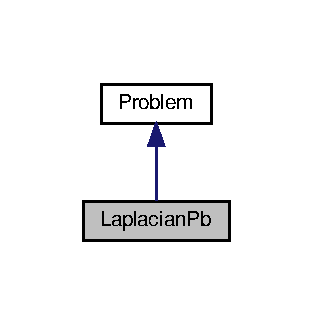
\includegraphics[width=150pt]{classLaplacianPb__inherit__graph}
\end{center}
\end{figure}


Collaboration diagram for Laplacian\+Pb\+:
\nopagebreak
\begin{figure}[H]
\begin{center}
\leavevmode
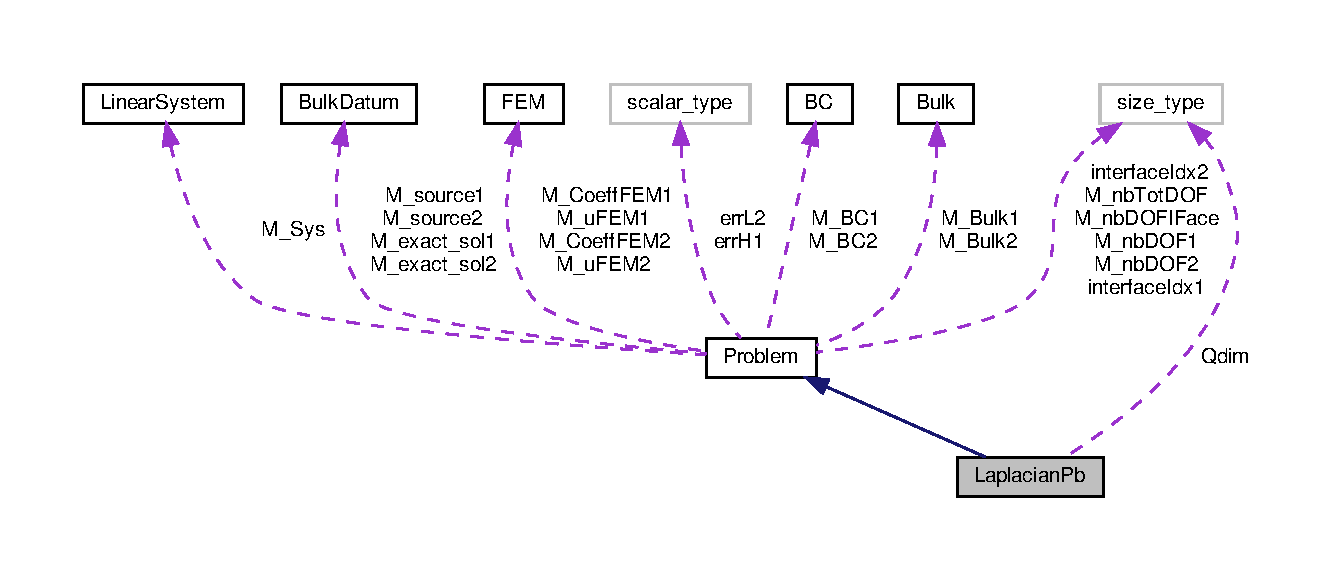
\includegraphics[width=350pt]{classLaplacianPb__coll__graph}
\end{center}
\end{figure}
\subsection*{Public Member Functions}
\begin{DoxyCompactItemize}
\item 
\mbox{\Hypertarget{classLaplacianPb_a23d66dc47132d2e44b7a7ab4194e60be}\label{classLaplacianPb_a23d66dc47132d2e44b7a7ab4194e60be}} 
{\bfseries Laplacian\+Pb} (Get\+Pot const \&data\+File, \hyperlink{classBulk}{Bulk} \&bulk1, \hyperlink{classBulk}{Bulk} \&bulk2, \hyperlink{classLinearSystem}{Linear\+System} \&ext\+Sys)
\item 
\mbox{\Hypertarget{classLaplacianPb_aa8baaaebc51fdb33f1e4ec3b810efc56}\label{classLaplacianPb_aa8baaaebc51fdb33f1e4ec3b810efc56}} 
void {\bfseries assemble\+Matrix} () override
\end{DoxyCompactItemize}
\subsection*{Static Public Attributes}
\begin{DoxyCompactItemize}
\item 
\mbox{\Hypertarget{classLaplacianPb_abcc44611e8914f470d51b1a15888cf29}\label{classLaplacianPb_abcc44611e8914f470d51b1a15888cf29}} 
static const size\+\_\+type {\bfseries Qdim} = 1
\end{DoxyCompactItemize}
\subsection*{Additional Inherited Members}


The documentation for this class was generated from the following file\+:\begin{DoxyCompactItemize}
\item 
include/Laplacian\+Pb.\+h\end{DoxyCompactItemize}

\hypertarget{classLinearElasticityPb}{}\section{Linear\+Elasticity\+Pb Class Reference}
\label{classLinearElasticityPb}\index{Linear\+Elasticity\+Pb@{Linear\+Elasticity\+Pb}}


Inheritance diagram for Linear\+Elasticity\+Pb\+:
\nopagebreak
\begin{figure}[H]
\begin{center}
\leavevmode
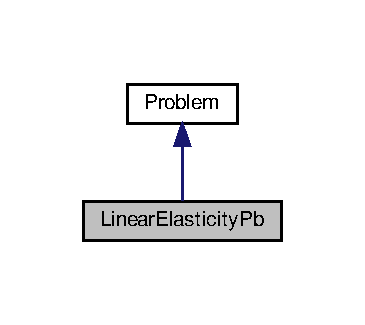
\includegraphics[width=175pt]{classLinearElasticityPb__inherit__graph}
\end{center}
\end{figure}


Collaboration diagram for Linear\+Elasticity\+Pb\+:
\nopagebreak
\begin{figure}[H]
\begin{center}
\leavevmode
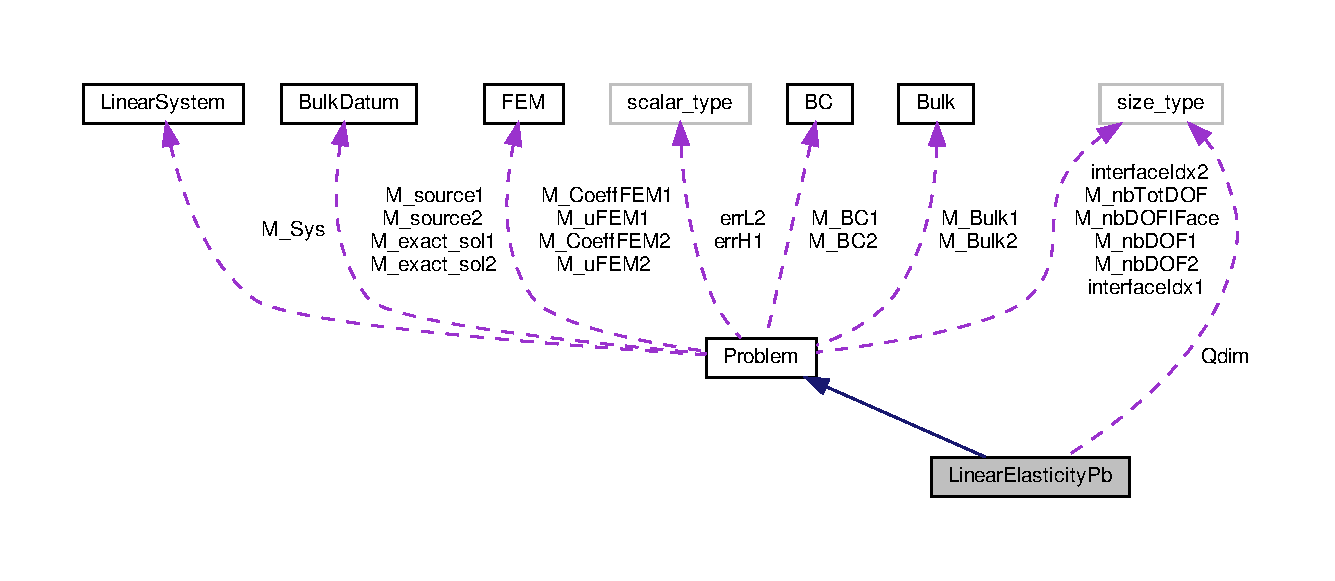
\includegraphics[width=350pt]{classLinearElasticityPb__coll__graph}
\end{center}
\end{figure}
\subsection*{Public Member Functions}
\begin{DoxyCompactItemize}
\item 
\mbox{\Hypertarget{classLinearElasticityPb_af8d7c56431cbf30079030183f2c77009}\label{classLinearElasticityPb_af8d7c56431cbf30079030183f2c77009}} 
{\bfseries Linear\+Elasticity\+Pb} (Get\+Pot const \&data\+File, \hyperlink{classBulk}{Bulk} \&bulk1, \hyperlink{classBulk}{Bulk} \&bulk2, \hyperlink{classLinearSystem}{Linear\+System} \&ext\+Sys)
\item 
\mbox{\Hypertarget{classLinearElasticityPb_a354738a6947854e0d64685cc8fe86fdf}\label{classLinearElasticityPb_a354738a6947854e0d64685cc8fe86fdf}} 
void {\bfseries assemble\+Matrix} () override
\end{DoxyCompactItemize}
\subsection*{Static Public Attributes}
\begin{DoxyCompactItemize}
\item 
\mbox{\Hypertarget{classLinearElasticityPb_a81612404c74ed25325041b3b27139529}\label{classLinearElasticityPb_a81612404c74ed25325041b3b27139529}} 
static const size\+\_\+type {\bfseries Qdim} = 2
\end{DoxyCompactItemize}
\subsection*{Additional Inherited Members}


The documentation for this class was generated from the following file\+:\begin{DoxyCompactItemize}
\item 
include/Linear\+Elasticity\+Pb.\+h\end{DoxyCompactItemize}

\hypertarget{classLinearSystem}{}\section{Linear\+System Class Reference}
\label{classLinearSystem}\index{Linear\+System@{Linear\+System}}
\subsection*{Public Member Functions}
\begin{DoxyCompactItemize}
\item 
\mbox{\Hypertarget{classLinearSystem_a9f1a7a6a3d1dc009fb8650d5ca3a0077}\label{classLinearSystem_a9f1a7a6a3d1dc009fb8650d5ca3a0077}} 
void {\bfseries add\+To\+Matrix} (int ndof)
\item 
\mbox{\Hypertarget{classLinearSystem_acf577d804361e6841a7710b706978417}\label{classLinearSystem_acf577d804361e6841a7710b706978417}} 
void {\bfseries copy\+Sub\+Matrix} (sparse\+Matrix\+Ptr\+\_\+\+Type source, int first\+\_\+row, int first\+\_\+column, scalar\+\_\+type scale=1.\+0, bool transpose=false)
\item 
\mbox{\Hypertarget{classLinearSystem_ad5025705b523e61b058f44a8a39d203d}\label{classLinearSystem_ad5025705b523e61b058f44a8a39d203d}} 
void {\bfseries add\+Sub\+Matrix} (sparse\+Matrix\+Ptr\+\_\+\+Type source, int first\+\_\+row, int first\+\_\+column, scalar\+\_\+type scale=1.\+0, bool transpose=false)
\item 
\mbox{\Hypertarget{classLinearSystem_a4f671c00a0c5a50965524cd9f28a3a30}\label{classLinearSystem_a4f671c00a0c5a50965524cd9f28a3a30}} 
void {\bfseries extract\+Sub\+Matrix} (sparse\+Matrix\+Ptr\+\_\+\+Type destination, int first\+\_\+row, int number\+\_\+rows, int first\+\_\+column, int number\+\_\+cols) const
\item 
\mbox{\Hypertarget{classLinearSystem_a2509c46a5c1f88fe68227f606a4b85ca}\label{classLinearSystem_a2509c46a5c1f88fe68227f606a4b85ca}} 
void {\bfseries copy\+Sub\+Vector} (scalar\+Vector\+Ptr\+\_\+\+Type source, int first\+\_\+row, scalar\+\_\+type scale=1.\+0)
\item 
\mbox{\Hypertarget{classLinearSystem_a2bc3f8fae6a408d159b1e66b5896d0e1}\label{classLinearSystem_a2bc3f8fae6a408d159b1e66b5896d0e1}} 
void {\bfseries add\+Sub\+Vector} (scalar\+Vector\+Ptr\+\_\+\+Type source, int first\+\_\+row, scalar\+\_\+type scale=1.\+0)
\item 
\mbox{\Hypertarget{classLinearSystem_ab4050b7fdf4b9dca260dabb27f82fb2d}\label{classLinearSystem_ab4050b7fdf4b9dca260dabb27f82fb2d}} 
void {\bfseries extract\+Sub\+Vector} (scalar\+Vector\+Ptr\+\_\+\+Type destination, int first\+\_\+row, std\+::string where=\char`\"{}sol\char`\"{}) const
\item 
\mbox{\Hypertarget{classLinearSystem_a5296d829ff117f6c70e17f277f7c0f43}\label{classLinearSystem_a5296d829ff117f6c70e17f277f7c0f43}} 
void {\bfseries extract\+Sub\+Vector} (scalar\+Vector\+\_\+\+Type \&destination, int first\+\_\+row, std\+::string where=\char`\"{}sol\char`\"{}) const
\item 
\mbox{\Hypertarget{classLinearSystem_a0e0a75162a3c1ebd08e5f49e43e05d6e}\label{classLinearSystem_a0e0a75162a3c1ebd08e5f49e43e05d6e}} 
sparse\+Matrix\+Ptr\+\_\+\+Type {\bfseries get\+Matrix} () const
\item 
\mbox{\Hypertarget{classLinearSystem_a83abf03b51dee2aac566f87fa3473bc0}\label{classLinearSystem_a83abf03b51dee2aac566f87fa3473bc0}} 
scalar\+Vector\+Ptr\+\_\+\+Type {\bfseries get\+R\+HS} () const
\item 
\mbox{\Hypertarget{classLinearSystem_a3ef7e07ffe4a2eeac49dbd8d48792df4}\label{classLinearSystem_a3ef7e07ffe4a2eeac49dbd8d48792df4}} 
scalar\+Vector\+Ptr\+\_\+\+Type {\bfseries get\+Sol} () const
\item 
\mbox{\Hypertarget{classLinearSystem_a07e9e5d259c3b3d3ddf71e4de1410bc9}\label{classLinearSystem_a07e9e5d259c3b3d3ddf71e4de1410bc9}} 
void {\bfseries add\+Sub\+System} (\hyperlink{classLinearSystem}{Linear\+System} $\ast$small, size\+\_\+type shift\+Rows, size\+\_\+type shift\+Columns)
\item 
\mbox{\Hypertarget{classLinearSystem_a477274ae086a3c851ae9b01e4dc4f327}\label{classLinearSystem_a477274ae086a3c851ae9b01e4dc4f327}} 
void {\bfseries solve} ()
\item 
\mbox{\Hypertarget{classLinearSystem_ae840d279eec2092a822f3f2e4f5bd091}\label{classLinearSystem_ae840d279eec2092a822f3f2e4f5bd091}} 
void {\bfseries compute\+Inverse} ()
\item 
\mbox{\Hypertarget{classLinearSystem_a1f17216367dfbc35e631fca351a4e71c}\label{classLinearSystem_a1f17216367dfbc35e631fca351a4e71c}} 
void {\bfseries save\+Matrix} (const char $\ast$nomefile=\char`\"{}Matrix.\+mm\char`\"{}) const
\item 
\mbox{\Hypertarget{classLinearSystem_afdff2fbf87f2428ade63a702eb6ef77f}\label{classLinearSystem_afdff2fbf87f2428ade63a702eb6ef77f}} 
void {\bfseries mult\+Add\+To\+R\+HS} (scalar\+Vector\+Ptr\+\_\+\+Type V, int first\+\_\+row, int first\+\_\+column, int nrows, int ncols)
\item 
\mbox{\Hypertarget{classLinearSystem_aa2a59e6468778d3c655299065876f769}\label{classLinearSystem_aa2a59e6468778d3c655299065876f769}} 
void {\bfseries mult\+Add\+To\+R\+HS} (sparse\+Matrix\+Ptr\+\_\+\+Type M, scalar\+Vector\+Ptr\+\_\+\+Type V, int first\+\_\+row\+Vector, int first\+\_\+row\+R\+HS, scalar\+\_\+type scale=1.\+0, bool transposed=false)
\item 
\mbox{\Hypertarget{classLinearSystem_a13451139fc04cc34d025fcb5b053ae01}\label{classLinearSystem_a13451139fc04cc34d025fcb5b053ae01}} 
void {\bfseries mult\+Add\+To\+R\+HS} (sparse\+Matrix\+Ptr\+\_\+\+Type M, scalar\+Vector\+\_\+\+Type \&V, int first\+\_\+row\+Vector, int first\+\_\+row\+R\+HS, scalar\+\_\+type scale=1.\+0, bool transposed=false)
\item 
\mbox{\Hypertarget{classLinearSystem_ad0577e81afa8dcc07db6806cb081192d}\label{classLinearSystem_ad0577e81afa8dcc07db6806cb081192d}} 
void {\bfseries clean\+R\+HS} ()
\item 
\mbox{\Hypertarget{classLinearSystem_a47007e77f2380ea08f0cb79377d06733}\label{classLinearSystem_a47007e77f2380ea08f0cb79377d06733}} 
void {\bfseries clean\+M\+AT} ()
\item 
\mbox{\Hypertarget{classLinearSystem_ae72aaec2e50c88fc5fabf9de8b4890ca}\label{classLinearSystem_ae72aaec2e50c88fc5fabf9de8b4890ca}} 
void {\bfseries set\+Null\+Row} (size\+\_\+type which)
\item 
\mbox{\Hypertarget{classLinearSystem_a2397eabd867ff7912e373757956d6beb}\label{classLinearSystem_a2397eabd867ff7912e373757956d6beb}} 
void {\bfseries set\+Matrix\+Value} (size\+\_\+type i, size\+\_\+type j, scalar\+\_\+type value)
\item 
\mbox{\Hypertarget{classLinearSystem_ad3688699408a10cbd533af5b0560881a}\label{classLinearSystem_ad3688699408a10cbd533af5b0560881a}} 
void {\bfseries set\+R\+H\+S\+Value} (size\+\_\+type i, scalar\+\_\+type value)
\end{DoxyCompactItemize}


The documentation for this class was generated from the following file\+:\begin{DoxyCompactItemize}
\item 
include/Linear\+System.\+h\end{DoxyCompactItemize}

\hypertarget{classLifeV_1_1Parser}{}\section{LifeV\+:\+:Parser Class Reference}
\label{classLifeV_1_1Parser}\index{Life\+V\+::\+Parser@{Life\+V\+::\+Parser}}


\hyperlink{classLifeV_1_1Parser}{Parser} -\/ A string parser for algebraic expressions.  




{\ttfamily \#include $<$Parser.\+h$>$}

\subsection*{Public Types}
\begin{Indent}\textbf{ Public Types}\par
\begin{DoxyCompactItemize}
\item 
\mbox{\Hypertarget{classLifeV_1_1Parser_af87d4a11879da16a0bba7bf81f98b957}\label{classLifeV_1_1Parser_af87d4a11879da16a0bba7bf81f98b957}} 
typedef std\+::vector$<$ std\+::string $>$ {\bfseries strings\+Vector\+\_\+\+Type}
\item 
\mbox{\Hypertarget{classLifeV_1_1Parser_a9491c77a9093b41468ca54b865c893ff}\label{classLifeV_1_1Parser_a9491c77a9093b41468ca54b865c893ff}} 
typedef std\+::string\+::const\+\_\+iterator {\bfseries string\+Iterator\+\_\+\+Type}
\item 
\mbox{\Hypertarget{classLifeV_1_1Parser_ae9a67e24d777a1f962026f5e1274b61a}\label{classLifeV_1_1Parser_ae9a67e24d777a1f962026f5e1274b61a}} 
typedef \hyperlink{classLifeV_1_1ParserSpiritGrammar}{Parser\+Spirit\+Grammar}$<$ string\+Iterator\+\_\+\+Type $>$ {\bfseries calculator\+\_\+\+Type}
\item 
\mbox{\Hypertarget{classLifeV_1_1Parser_a9e5861cc337d7534e8641b1709d193db}\label{classLifeV_1_1Parser_a9e5861cc337d7534e8641b1709d193db}} 
typedef calculator\+\_\+\+Type\+::results\+\_\+\+Type {\bfseries results\+\_\+\+Type}
\end{DoxyCompactItemize}
\end{Indent}
\subsection*{Public Member Functions}
\begin{Indent}\textbf{ Constructors \& Destructor}\par
\begin{DoxyCompactItemize}
\item 
\mbox{\Hypertarget{classLifeV_1_1Parser_a439ecd746d503e75b6e07f2933a665dc}\label{classLifeV_1_1Parser_a439ecd746d503e75b6e07f2933a665dc}} 
\hyperlink{classLifeV_1_1Parser_a439ecd746d503e75b6e07f2933a665dc}{Parser} ()
\begin{DoxyCompactList}\small\item\em Empty constructor (it needs a manual call to set\+String) \end{DoxyCompactList}\item 
\hyperlink{classLifeV_1_1Parser_a6acf25b7222f0c65d1414611236d1820}{Parser} (const std\+::string \&string)
\begin{DoxyCompactList}\small\item\em Constructor. \end{DoxyCompactList}\item 
\hyperlink{classLifeV_1_1Parser_a0f7c4d10928fd2139e76baf44996b610}{Parser} (const \hyperlink{classLifeV_1_1Parser}{Parser} \&parser)
\begin{DoxyCompactList}\small\item\em Copy constructor. \end{DoxyCompactList}\item 
\mbox{\Hypertarget{classLifeV_1_1Parser_a34d16f77f23cf33b3bc3f8293ed0e2ed}\label{classLifeV_1_1Parser_a34d16f77f23cf33b3bc3f8293ed0e2ed}} 
virtual \hyperlink{classLifeV_1_1Parser_a34d16f77f23cf33b3bc3f8293ed0e2ed}{$\sim$\+Parser} ()
\begin{DoxyCompactList}\small\item\em Destructor. \end{DoxyCompactList}\end{DoxyCompactItemize}
\end{Indent}
\begin{Indent}\textbf{ Operators}\par
\begin{DoxyCompactItemize}
\item 
\hyperlink{classLifeV_1_1Parser}{Parser} \& \hyperlink{classLifeV_1_1Parser_a4dde1ca3f1f88623a91d8e498e274f52}{operator=} (const \hyperlink{classLifeV_1_1Parser}{Parser} \&parser)
\begin{DoxyCompactList}\small\item\em Operator =. \end{DoxyCompactList}\end{DoxyCompactItemize}
\end{Indent}
\begin{Indent}\textbf{ Methods}\par
\begin{DoxyCompactItemize}
\item 
const scalar\+\_\+type \& \hyperlink{classLifeV_1_1Parser_ac0e93cf8f4583c7c9f3c83990b4814a5}{evaluate} (const ID \&id=0)
\item 
U\+Int \hyperlink{classLifeV_1_1Parser_a37ae3af9abcf72ca8e1537ec771b523a}{count\+Substring} (const std\+::string \&substring)
\item 
\mbox{\Hypertarget{classLifeV_1_1Parser_acbc44ff1f0b0074f071ea264a95cb9e7}\label{classLifeV_1_1Parser_acbc44ff1f0b0074f071ea264a95cb9e7}} 
void \hyperlink{classLifeV_1_1Parser_acbc44ff1f0b0074f071ea264a95cb9e7}{clear\+Variables} ()
\begin{DoxyCompactList}\small\item\em Clear all the variables. \end{DoxyCompactList}\end{DoxyCompactItemize}
\end{Indent}
\begin{Indent}\textbf{ Set Methods}\par
\begin{DoxyCompactItemize}
\item 
void \hyperlink{classLifeV_1_1Parser_ac05769e836a0dc95d9c020df361a5194}{set\+String} (const std\+::string \&string, const std\+::string \&string\+Separator=\char`\"{};\char`\"{})
\item 
void \hyperlink{classLifeV_1_1Parser_a60ab2ac0a3a12770af9dc657ecbac38d}{set\+Variable} (const std\+::string \&name, const scalar\+\_\+type \&value)
\end{DoxyCompactItemize}
\end{Indent}
\begin{Indent}\textbf{ Get Methods}\par
\begin{DoxyCompactItemize}
\item 
const scalar\+\_\+type \& \hyperlink{classLifeV_1_1Parser_a2abb06796ab8b5968e824388b721427f}{variable} (const std\+::string \&name)
\end{DoxyCompactItemize}
\end{Indent}


\subsection{Detailed Description}
\hyperlink{classLifeV_1_1Parser}{Parser} -\/ A string parser for algebraic expressions. 

\begin{DoxyAuthor}{Author}
(s) Cristiano Malossi, Gilles Fourestey
\end{DoxyAuthor}
See {\ttfamily \hyperlink{classLifeV_1_1ParserSpiritGrammar}{Parser\+Spirit\+Grammar}} class for more details. 

\subsection{Constructor \& Destructor Documentation}
\mbox{\Hypertarget{classLifeV_1_1Parser_a6acf25b7222f0c65d1414611236d1820}\label{classLifeV_1_1Parser_a6acf25b7222f0c65d1414611236d1820}} 
\index{Life\+V\+::\+Parser@{Life\+V\+::\+Parser}!Parser@{Parser}}
\index{Parser@{Parser}!Life\+V\+::\+Parser@{Life\+V\+::\+Parser}}
\subsubsection{\texorpdfstring{Parser()}{Parser()}\hspace{0.1cm}{\footnotesize\ttfamily [1/2]}}
{\footnotesize\ttfamily Life\+V\+::\+Parser\+::\+Parser (\begin{DoxyParamCaption}\item[{const std\+::string \&}]{string }\end{DoxyParamCaption})\hspace{0.3cm}{\ttfamily [explicit]}}



Constructor. 


\begin{DoxyParams}{Parameters}
{\em string} & expression to parse \\
\hline
\end{DoxyParams}
\mbox{\Hypertarget{classLifeV_1_1Parser_a0f7c4d10928fd2139e76baf44996b610}\label{classLifeV_1_1Parser_a0f7c4d10928fd2139e76baf44996b610}} 
\index{Life\+V\+::\+Parser@{Life\+V\+::\+Parser}!Parser@{Parser}}
\index{Parser@{Parser}!Life\+V\+::\+Parser@{Life\+V\+::\+Parser}}
\subsubsection{\texorpdfstring{Parser()}{Parser()}\hspace{0.1cm}{\footnotesize\ttfamily [2/2]}}
{\footnotesize\ttfamily Life\+V\+::\+Parser\+::\+Parser (\begin{DoxyParamCaption}\item[{const \hyperlink{classLifeV_1_1Parser}{Parser} \&}]{parser }\end{DoxyParamCaption})\hspace{0.3cm}{\ttfamily [explicit]}}



Copy constructor. 


\begin{DoxyParams}{Parameters}
{\em parser} & \hyperlink{classLifeV_1_1Parser}{Parser} \\
\hline
\end{DoxyParams}


\subsection{Member Function Documentation}
\mbox{\Hypertarget{classLifeV_1_1Parser_a37ae3af9abcf72ca8e1537ec771b523a}\label{classLifeV_1_1Parser_a37ae3af9abcf72ca8e1537ec771b523a}} 
\index{Life\+V\+::\+Parser@{Life\+V\+::\+Parser}!count\+Substring@{count\+Substring}}
\index{count\+Substring@{count\+Substring}!Life\+V\+::\+Parser@{Life\+V\+::\+Parser}}
\subsubsection{\texorpdfstring{count\+Substring()}{countSubstring()}}
{\footnotesize\ttfamily U\+Int Life\+V\+::\+Parser\+::count\+Substring (\begin{DoxyParamCaption}\item[{const std\+::string \&}]{substring }\end{DoxyParamCaption})}

Count how many times a substring is present in the string (utility for B\+C\+Interface\+Function)


\begin{DoxyParams}{Parameters}
{\em substring} & string to find \\
\hline
\end{DoxyParams}
\begin{DoxyReturn}{Returns}
number of substring 
\end{DoxyReturn}
\mbox{\Hypertarget{classLifeV_1_1Parser_ac0e93cf8f4583c7c9f3c83990b4814a5}\label{classLifeV_1_1Parser_ac0e93cf8f4583c7c9f3c83990b4814a5}} 
\index{Life\+V\+::\+Parser@{Life\+V\+::\+Parser}!evaluate@{evaluate}}
\index{evaluate@{evaluate}!Life\+V\+::\+Parser@{Life\+V\+::\+Parser}}
\subsubsection{\texorpdfstring{evaluate()}{evaluate()}}
{\footnotesize\ttfamily const scalar\+\_\+type\& Life\+V\+::\+Parser\+::evaluate (\begin{DoxyParamCaption}\item[{const ID \&}]{id = {\ttfamily 0} }\end{DoxyParamCaption})}

Evaluate the expression 
\begin{DoxyParams}{Parameters}
{\em id} & expression index (starting from 0) \\
\hline
\end{DoxyParams}
\begin{DoxyReturn}{Returns}
computed value 
\end{DoxyReturn}
\mbox{\Hypertarget{classLifeV_1_1Parser_a4dde1ca3f1f88623a91d8e498e274f52}\label{classLifeV_1_1Parser_a4dde1ca3f1f88623a91d8e498e274f52}} 
\index{Life\+V\+::\+Parser@{Life\+V\+::\+Parser}!operator=@{operator=}}
\index{operator=@{operator=}!Life\+V\+::\+Parser@{Life\+V\+::\+Parser}}
\subsubsection{\texorpdfstring{operator=()}{operator=()}}
{\footnotesize\ttfamily \hyperlink{classLifeV_1_1Parser}{Parser}\& Life\+V\+::\+Parser\+::operator= (\begin{DoxyParamCaption}\item[{const \hyperlink{classLifeV_1_1Parser}{Parser} \&}]{parser }\end{DoxyParamCaption})}



Operator =. 


\begin{DoxyParams}{Parameters}
{\em parser} & \hyperlink{classLifeV_1_1Parser}{Parser} \\
\hline
\end{DoxyParams}
\begin{DoxyReturn}{Returns}
reference to a copy of the class 
\end{DoxyReturn}
\mbox{\Hypertarget{classLifeV_1_1Parser_ac05769e836a0dc95d9c020df361a5194}\label{classLifeV_1_1Parser_ac05769e836a0dc95d9c020df361a5194}} 
\index{Life\+V\+::\+Parser@{Life\+V\+::\+Parser}!set\+String@{set\+String}}
\index{set\+String@{set\+String}!Life\+V\+::\+Parser@{Life\+V\+::\+Parser}}
\subsubsection{\texorpdfstring{set\+String()}{setString()}}
{\footnotesize\ttfamily void Life\+V\+::\+Parser\+::set\+String (\begin{DoxyParamCaption}\item[{const std\+::string \&}]{string,  }\item[{const std\+::string \&}]{string\+Separator = {\ttfamily \char`\"{};\char`\"{}} }\end{DoxyParamCaption})}

Set string function


\begin{DoxyParams}{Parameters}
{\em string} & Expression to evaluate \\
\hline
{\em string\+Separator} & Separator identifier (default -\/$>$ \char`\"{};\char`\"{}) \\
\hline
\end{DoxyParams}
\mbox{\Hypertarget{classLifeV_1_1Parser_a60ab2ac0a3a12770af9dc657ecbac38d}\label{classLifeV_1_1Parser_a60ab2ac0a3a12770af9dc657ecbac38d}} 
\index{Life\+V\+::\+Parser@{Life\+V\+::\+Parser}!set\+Variable@{set\+Variable}}
\index{set\+Variable@{set\+Variable}!Life\+V\+::\+Parser@{Life\+V\+::\+Parser}}
\subsubsection{\texorpdfstring{set\+Variable()}{setVariable()}}
{\footnotesize\ttfamily void Life\+V\+::\+Parser\+::set\+Variable (\begin{DoxyParamCaption}\item[{const std\+::string \&}]{name,  }\item[{const scalar\+\_\+type \&}]{value }\end{DoxyParamCaption})}

Set/replace a variable


\begin{DoxyParams}{Parameters}
{\em name} & name of the parameter \\
\hline
{\em value} & value of the parameter \\
\hline
\end{DoxyParams}
\mbox{\Hypertarget{classLifeV_1_1Parser_a2abb06796ab8b5968e824388b721427f}\label{classLifeV_1_1Parser_a2abb06796ab8b5968e824388b721427f}} 
\index{Life\+V\+::\+Parser@{Life\+V\+::\+Parser}!variable@{variable}}
\index{variable@{variable}!Life\+V\+::\+Parser@{Life\+V\+::\+Parser}}
\subsubsection{\texorpdfstring{variable()}{variable()}}
{\footnotesize\ttfamily const scalar\+\_\+type\& Life\+V\+::\+Parser\+::variable (\begin{DoxyParamCaption}\item[{const std\+::string \&}]{name }\end{DoxyParamCaption})}

Get variable


\begin{DoxyParams}{Parameters}
{\em name} & name of the parameter \\
\hline
\end{DoxyParams}
\begin{DoxyReturn}{Returns}
value of the variable 
\end{DoxyReturn}


The documentation for this class was generated from the following file\+:\begin{DoxyCompactItemize}
\item 
include/\hyperlink{Parser_8h}{Parser.\+h}\end{DoxyCompactItemize}

\hypertarget{classLifeV_1_1ParserSpiritGrammar}{}\section{LifeV\+:\+:Parser\+Spirit\+Grammar$<$ Iterator\+Type, Results\+Type $>$ Class Template Reference}
\label{classLifeV_1_1ParserSpiritGrammar}\index{Life\+V\+::\+Parser\+Spirit\+Grammar$<$ Iterator\+Type, Results\+Type $>$@{Life\+V\+::\+Parser\+Spirit\+Grammar$<$ Iterator\+Type, Results\+Type $>$}}


\hyperlink{classLifeV_1_1ParserSpiritGrammar}{Parser\+Spirit\+Grammar} -\/ A string parser grammar based on {\ttfamily boost\+::spirit\+::qi}.  




{\ttfamily \#include $<$Parser\+Spirit\+Grammar.\+h$>$}



Inheritance diagram for LifeV\+:\+:Parser\+Spirit\+Grammar$<$ Iterator\+Type, Results\+Type $>$\+:
\nopagebreak
\begin{figure}[H]
\begin{center}
\leavevmode
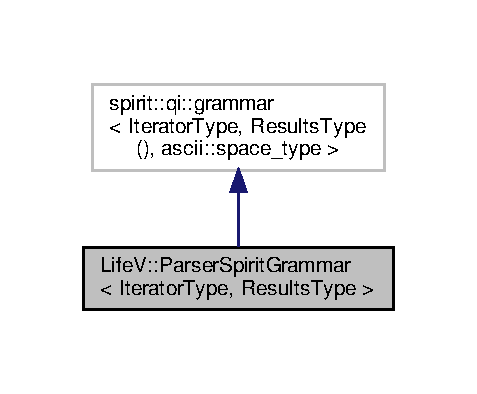
\includegraphics[width=229pt]{classLifeV_1_1ParserSpiritGrammar__inherit__graph}
\end{center}
\end{figure}


Collaboration diagram for LifeV\+:\+:Parser\+Spirit\+Grammar$<$ Iterator\+Type, Results\+Type $>$\+:
\nopagebreak
\begin{figure}[H]
\begin{center}
\leavevmode
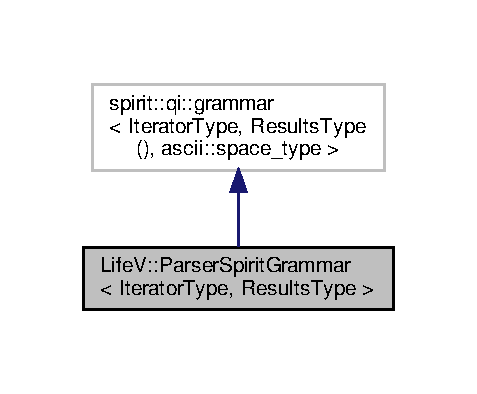
\includegraphics[width=229pt]{classLifeV_1_1ParserSpiritGrammar__coll__graph}
\end{center}
\end{figure}
\subsection*{Public Types}
\begin{Indent}\textbf{ Public Types}\par
\begin{DoxyCompactItemize}
\item 
\mbox{\Hypertarget{classLifeV_1_1ParserSpiritGrammar_aaa28e2ed8f68d686da1e0bcc5834ed3b}\label{classLifeV_1_1ParserSpiritGrammar_aaa28e2ed8f68d686da1e0bcc5834ed3b}} 
typedef Iterator\+Type {\bfseries iterator\+\_\+\+Type}
\item 
\mbox{\Hypertarget{classLifeV_1_1ParserSpiritGrammar_a8aca47ceac2876986dbc2ff9ee4d2edd}\label{classLifeV_1_1ParserSpiritGrammar_a8aca47ceac2876986dbc2ff9ee4d2edd}} 
typedef boost\+::iterator\+\_\+range$<$ iterator\+\_\+\+Type $>$ {\bfseries iterator\+Range\+\_\+\+Type}
\item 
\mbox{\Hypertarget{classLifeV_1_1ParserSpiritGrammar_a98dabec1a4a9a743a1d3b35e994cec7c}\label{classLifeV_1_1ParserSpiritGrammar_a98dabec1a4a9a743a1d3b35e994cec7c}} 
typedef Results\+Type {\bfseries results\+\_\+\+Type}
\end{DoxyCompactItemize}
\end{Indent}
\subsection*{Public Member Functions}
\begin{Indent}\textbf{ Constructors \& Destructor}\par
\begin{DoxyCompactItemize}
\item 
\mbox{\Hypertarget{classLifeV_1_1ParserSpiritGrammar_afd12d0ca36622930f0c5e574c96acaa7}\label{classLifeV_1_1ParserSpiritGrammar_afd12d0ca36622930f0c5e574c96acaa7}} 
\hyperlink{classLifeV_1_1ParserSpiritGrammar_afd12d0ca36622930f0c5e574c96acaa7}{Parser\+Spirit\+Grammar} ()
\begin{DoxyCompactList}\small\item\em Constructor. \end{DoxyCompactList}\item 
\hyperlink{classLifeV_1_1ParserSpiritGrammar_a2a0d8a4396ae61a66edc4f320d9e79f5}{Parser\+Spirit\+Grammar} (const \hyperlink{classLifeV_1_1ParserSpiritGrammar}{Parser\+Spirit\+Grammar} \&spirit\+Grammar)
\begin{DoxyCompactList}\small\item\em Copy constructor. \end{DoxyCompactList}\item 
\mbox{\Hypertarget{classLifeV_1_1ParserSpiritGrammar_a32c0629e6ee7ea37bb0b3159b0fa31ee}\label{classLifeV_1_1ParserSpiritGrammar_a32c0629e6ee7ea37bb0b3159b0fa31ee}} 
virtual \hyperlink{classLifeV_1_1ParserSpiritGrammar_a32c0629e6ee7ea37bb0b3159b0fa31ee}{$\sim$\+Parser\+Spirit\+Grammar} ()
\begin{DoxyCompactList}\small\item\em Destructor. \end{DoxyCompactList}\end{DoxyCompactItemize}
\end{Indent}
\begin{Indent}\textbf{ Operators}\par
\begin{DoxyCompactItemize}
\item 
\hyperlink{classLifeV_1_1ParserSpiritGrammar}{Parser\+Spirit\+Grammar} \& \hyperlink{classLifeV_1_1ParserSpiritGrammar_a6ce4fa32aacdc3bc7e4b38be901f94cf}{operator=} (const \hyperlink{classLifeV_1_1ParserSpiritGrammar}{Parser\+Spirit\+Grammar} \&spirit\+Grammar)
\begin{DoxyCompactList}\small\item\em Operator =. \end{DoxyCompactList}\end{DoxyCompactItemize}
\end{Indent}
\begin{Indent}\textbf{ Methods}\par
\begin{DoxyCompactItemize}
\item 
void \hyperlink{classLifeV_1_1ParserSpiritGrammar_a7ccdf51b58cd920a08d18adaea2524ca}{assign\+Variable} (const iterator\+Range\+\_\+\+Type \&string\+Iterator\+Range, const scalar\+\_\+type \&value)
\item 
\mbox{\Hypertarget{classLifeV_1_1ParserSpiritGrammar_a81b8e2abdda8a35738367f2dcfb69c75}\label{classLifeV_1_1ParserSpiritGrammar_a81b8e2abdda8a35738367f2dcfb69c75}} 
void \hyperlink{classLifeV_1_1ParserSpiritGrammar_a81b8e2abdda8a35738367f2dcfb69c75}{clear\+Variables} ()
\begin{DoxyCompactList}\small\item\em Clear all the variables. \end{DoxyCompactList}\end{DoxyCompactItemize}
\end{Indent}
\begin{Indent}\textbf{ Set Methods}\par
\begin{DoxyCompactItemize}
\item 
\mbox{\Hypertarget{classLifeV_1_1ParserSpiritGrammar_aa48cdca46ab32d3c1e55e656aa82e902}\label{classLifeV_1_1ParserSpiritGrammar_aa48cdca46ab32d3c1e55e656aa82e902}} 
void \hyperlink{classLifeV_1_1ParserSpiritGrammar_aa48cdca46ab32d3c1e55e656aa82e902}{set\+Default\+Variables} ()
\begin{DoxyCompactList}\small\item\em Set default variables. \end{DoxyCompactList}\item 
void \hyperlink{classLifeV_1_1ParserSpiritGrammar_add7ee83b39ebf408710c820a4365eafa}{set\+Variable} (const std\+::string \&name, const scalar\+\_\+type \&value)
\end{DoxyCompactItemize}
\end{Indent}
\begin{Indent}\textbf{ Get Methods}\par
\begin{DoxyCompactItemize}
\item 
scalar\+\_\+type \& \hyperlink{classLifeV_1_1ParserSpiritGrammar_a53ba937b8359b093d650d1a907d7b738}{variable} (const std\+::string \&name)
\end{DoxyCompactItemize}
\end{Indent}


\subsection{Detailed Description}
\subsubsection*{template$<$typename Iterator\+Type = std\+::string\+::const\+\_\+iterator, typename Results\+Type = std\+::vector $<$ scalar\+\_\+type $>$$>$\newline
class Life\+V\+::\+Parser\+Spirit\+Grammar$<$ Iterator\+Type, Results\+Type $>$}

\hyperlink{classLifeV_1_1ParserSpiritGrammar}{Parser\+Spirit\+Grammar} -\/ A string parser grammar based on {\ttfamily boost\+::spirit\+::qi}. 

\begin{DoxyAuthor}{Author}
(s) Cristiano Malossi
\end{DoxyAuthor}
{\ttfamily \hyperlink{classLifeV_1_1ParserSpiritGrammar}{Parser\+Spirit\+Grammar}} is a {\ttfamily boost\+::spirit\+::qi} based class to perform evaluation of {\ttfamily std\+::string} expressions.

{\bfseries E\+X\+A\+M\+P\+LE -\/ H\+OW TO U\+SE} Let\textquotesingle{}s consider the following example\+: suppose that we have this function\+:

\mbox{[}u,v,w\mbox{]} = f(x,y,z,t)

where

u(x) = a$\ast$b$\ast$x v(x,y) = a/b$\ast$sqrt(x$^\wedge$2 + y$^\wedge$2) w(t) = b$\ast$t;

with \char`\"{}a\char`\"{} and \char`\"{}b\char`\"{} constants such that a=5.\+12345, b=9.\+999999.

To evaluate function f(x,y,z,t), we use this syntax\+:

string = \char`\"{}a=5.\+12345 ; b=9.\+999999 ; (a$\ast$b$\ast$x, a/b$\ast$sqrt(x$^\wedge$2 + y$^\wedge$2), b$\ast$t)\char`\"{}

where semicolons (\char`\"{};\char`\"{}) separate constants and commas (\char`\"{},\char`\"{}) separate output functions.

N\+O\+TE\+: Currently \hyperlink{classLifeV_1_1ParserSpiritGrammar}{Parser\+Spirit\+Grammar} works with the following operators\+: \begin{DoxyVerb}*  +, -, *, /, ^, sqrt(), sin(), cos(), tan(), exp(), log(), log10(), >, <.
*  \end{DoxyVerb}
 

\subsection{Constructor \& Destructor Documentation}
\mbox{\Hypertarget{classLifeV_1_1ParserSpiritGrammar_a2a0d8a4396ae61a66edc4f320d9e79f5}\label{classLifeV_1_1ParserSpiritGrammar_a2a0d8a4396ae61a66edc4f320d9e79f5}} 
\index{Life\+V\+::\+Parser\+Spirit\+Grammar@{Life\+V\+::\+Parser\+Spirit\+Grammar}!Parser\+Spirit\+Grammar@{Parser\+Spirit\+Grammar}}
\index{Parser\+Spirit\+Grammar@{Parser\+Spirit\+Grammar}!Life\+V\+::\+Parser\+Spirit\+Grammar@{Life\+V\+::\+Parser\+Spirit\+Grammar}}
\subsubsection{\texorpdfstring{Parser\+Spirit\+Grammar()}{ParserSpiritGrammar()}}
{\footnotesize\ttfamily template$<$typename Iterator\+Type , typename Results\+Type $>$ \\
\hyperlink{classLifeV_1_1ParserSpiritGrammar}{Life\+V\+::\+Parser\+Spirit\+Grammar}$<$ Iterator\+Type, Results\+Type $>$\+::\hyperlink{classLifeV_1_1ParserSpiritGrammar}{Parser\+Spirit\+Grammar} (\begin{DoxyParamCaption}\item[{const \hyperlink{classLifeV_1_1ParserSpiritGrammar}{Parser\+Spirit\+Grammar}$<$ Iterator\+Type, Results\+Type $>$ \&}]{spirit\+Grammar }\end{DoxyParamCaption})\hspace{0.3cm}{\ttfamily [explicit]}}



Copy constructor. 


\begin{DoxyParams}{Parameters}
{\em \hyperlink{classLifeV_1_1ParserSpiritGrammar}{Parser\+Spirit\+Grammar}} & \hyperlink{classLifeV_1_1ParserSpiritGrammar}{Parser\+Spirit\+Grammar} \\
\hline
\end{DoxyParams}


\subsection{Member Function Documentation}
\mbox{\Hypertarget{classLifeV_1_1ParserSpiritGrammar_a7ccdf51b58cd920a08d18adaea2524ca}\label{classLifeV_1_1ParserSpiritGrammar_a7ccdf51b58cd920a08d18adaea2524ca}} 
\index{Life\+V\+::\+Parser\+Spirit\+Grammar@{Life\+V\+::\+Parser\+Spirit\+Grammar}!assign\+Variable@{assign\+Variable}}
\index{assign\+Variable@{assign\+Variable}!Life\+V\+::\+Parser\+Spirit\+Grammar@{Life\+V\+::\+Parser\+Spirit\+Grammar}}
\subsubsection{\texorpdfstring{assign\+Variable()}{assignVariable()}}
{\footnotesize\ttfamily template$<$typename Iterator\+Type = std\+::string\+::const\+\_\+iterator, typename Results\+Type = std\+::vector $<$ scalar\+\_\+type $>$$>$ \\
void \hyperlink{classLifeV_1_1ParserSpiritGrammar}{Life\+V\+::\+Parser\+Spirit\+Grammar}$<$ Iterator\+Type, Results\+Type $>$\+::assign\+Variable (\begin{DoxyParamCaption}\item[{const iterator\+Range\+\_\+\+Type \&}]{string\+Iterator\+Range,  }\item[{const scalar\+\_\+type \&}]{value }\end{DoxyParamCaption})\hspace{0.3cm}{\ttfamily [inline]}}

Assign a variable using a {\ttfamily boost\+::iterator\+\_\+range} 


\begin{DoxyParams}{Parameters}
{\em string\+Iterator\+Range} & name of the parameter \\
\hline
{\em value} & value of the parameter \\
\hline
\end{DoxyParams}
\mbox{\Hypertarget{classLifeV_1_1ParserSpiritGrammar_a6ce4fa32aacdc3bc7e4b38be901f94cf}\label{classLifeV_1_1ParserSpiritGrammar_a6ce4fa32aacdc3bc7e4b38be901f94cf}} 
\index{Life\+V\+::\+Parser\+Spirit\+Grammar@{Life\+V\+::\+Parser\+Spirit\+Grammar}!operator=@{operator=}}
\index{operator=@{operator=}!Life\+V\+::\+Parser\+Spirit\+Grammar@{Life\+V\+::\+Parser\+Spirit\+Grammar}}
\subsubsection{\texorpdfstring{operator=()}{operator=()}}
{\footnotesize\ttfamily template$<$typename Iterator\+Type , typename Results\+Type $>$ \\
\hyperlink{classLifeV_1_1ParserSpiritGrammar}{Parser\+Spirit\+Grammar}$<$ Iterator\+Type, Results\+Type $>$ \& \hyperlink{classLifeV_1_1ParserSpiritGrammar}{Life\+V\+::\+Parser\+Spirit\+Grammar}$<$ Iterator\+Type, Results\+Type $>$\+::operator= (\begin{DoxyParamCaption}\item[{const \hyperlink{classLifeV_1_1ParserSpiritGrammar}{Parser\+Spirit\+Grammar}$<$ Iterator\+Type, Results\+Type $>$ \&}]{spirit\+Grammar }\end{DoxyParamCaption})}



Operator =. 


\begin{DoxyParams}{Parameters}
{\em Spirit\+Grammar} & \hyperlink{classLifeV_1_1ParserSpiritGrammar}{Parser\+Spirit\+Grammar} \\
\hline
\end{DoxyParams}
\begin{DoxyReturn}{Returns}
reference to a copy of the class 
\end{DoxyReturn}
\mbox{\Hypertarget{classLifeV_1_1ParserSpiritGrammar_add7ee83b39ebf408710c820a4365eafa}\label{classLifeV_1_1ParserSpiritGrammar_add7ee83b39ebf408710c820a4365eafa}} 
\index{Life\+V\+::\+Parser\+Spirit\+Grammar@{Life\+V\+::\+Parser\+Spirit\+Grammar}!set\+Variable@{set\+Variable}}
\index{set\+Variable@{set\+Variable}!Life\+V\+::\+Parser\+Spirit\+Grammar@{Life\+V\+::\+Parser\+Spirit\+Grammar}}
\subsubsection{\texorpdfstring{set\+Variable()}{setVariable()}}
{\footnotesize\ttfamily template$<$typename Iterator\+Type , typename Results\+Type $>$ \\
void \hyperlink{classLifeV_1_1ParserSpiritGrammar}{Life\+V\+::\+Parser\+Spirit\+Grammar}$<$ Iterator\+Type, Results\+Type $>$\+::set\+Variable (\begin{DoxyParamCaption}\item[{const std\+::string \&}]{name,  }\item[{const scalar\+\_\+type \&}]{value }\end{DoxyParamCaption})\hspace{0.3cm}{\ttfamily [inline]}}

Set/replace a variable


\begin{DoxyParams}{Parameters}
{\em name} & name of the parameter \\
\hline
{\em value} & value of the parameter \\
\hline
\end{DoxyParams}
\mbox{\Hypertarget{classLifeV_1_1ParserSpiritGrammar_a53ba937b8359b093d650d1a907d7b738}\label{classLifeV_1_1ParserSpiritGrammar_a53ba937b8359b093d650d1a907d7b738}} 
\index{Life\+V\+::\+Parser\+Spirit\+Grammar@{Life\+V\+::\+Parser\+Spirit\+Grammar}!variable@{variable}}
\index{variable@{variable}!Life\+V\+::\+Parser\+Spirit\+Grammar@{Life\+V\+::\+Parser\+Spirit\+Grammar}}
\subsubsection{\texorpdfstring{variable()}{variable()}}
{\footnotesize\ttfamily template$<$typename Iterator\+Type = std\+::string\+::const\+\_\+iterator, typename Results\+Type = std\+::vector $<$ scalar\+\_\+type $>$$>$ \\
scalar\+\_\+type\& \hyperlink{classLifeV_1_1ParserSpiritGrammar}{Life\+V\+::\+Parser\+Spirit\+Grammar}$<$ Iterator\+Type, Results\+Type $>$\+::variable (\begin{DoxyParamCaption}\item[{const std\+::string \&}]{name }\end{DoxyParamCaption})\hspace{0.3cm}{\ttfamily [inline]}}

Get variable


\begin{DoxyParams}{Parameters}
{\em name} & name of the parameter \\
\hline
\end{DoxyParams}
\begin{DoxyReturn}{Returns}
value of the variable 
\end{DoxyReturn}


The documentation for this class was generated from the following file\+:\begin{DoxyCompactItemize}
\item 
include/\hyperlink{ParserSpiritGrammar_8h}{Parser\+Spirit\+Grammar.\+h}\end{DoxyCompactItemize}

\hypertarget{classProblem}{}\doxysection{Problem Class Reference}
\label{classProblem}\index{Problem@{Problem}}


Inheritance diagram for Problem\+:
% FIG 0


Collaboration diagram for Problem\+:
% FIG 1
\doxysubsection*{Public Member Functions}
\begin{DoxyCompactItemize}
\item 
\mbox{\hyperlink{classProblem_ae48369cd7f0fd844855055fde437b658}{Problem}} (Get\+Pot const \&data\+File, std\+::string const problem, \mbox{\hyperlink{classBulk}{Bulk}} \&bulk1, \mbox{\hyperlink{classBulk}{Bulk}} \&bulk2, const size\+\_\+type dim, \mbox{\hyperlink{classLinearSystem}{Linear\+System}} \&ext\+Sys)
\item 
\mbox{\Hypertarget{classProblem_aabf50a05ce09ac973c6f7baae0d79a36}\label{classProblem_aabf50a05ce09ac973c6f7baae0d79a36}} 
\mbox{\hyperlink{classFEM}{F\+EM}} {\bfseries get\+F\+EM} (size\+\_\+type const idx) const
\item 
\mbox{\Hypertarget{classProblem_a842e147eb80b8c0a4480804f5e13c501}\label{classProblem_a842e147eb80b8c0a4480804f5e13c501}} 
\mbox{\hyperlink{classLinearSystem}{Linear\+System}} \& {\bfseries get\+S\+YS} () const
\item 
\mbox{\Hypertarget{classProblem_a0778563987b8c77f26607869ae62f8e5}\label{classProblem_a0778563987b8c77f26607869ae62f8e5}} 
size\+\_\+type {\bfseries get\+N\+D\+OF} (std\+::string const variable=\char`\"{}all\char`\"{}) const
\item 
\mbox{\Hypertarget{classProblem_ad497cda7281ccc702dca456cb458160d}\label{classProblem_ad497cda7281ccc702dca456cb458160d}} 
scalar\+\_\+type {\bfseries get\+L2\+E\+RR} () const
\item 
\mbox{\Hypertarget{classProblem_a3f70e73a231833475bb495d657505196}\label{classProblem_a3f70e73a231833475bb495d657505196}} 
scalar\+\_\+type {\bfseries get\+H1\+E\+RR} () const
\item 
virtual void \mbox{\hyperlink{classProblem_a834cfdf8d3909ad602712989dccac7c9}{assemble\+Matrix}} ()=0
\item 
virtual void \mbox{\hyperlink{classProblem_a40a120364978bcd6286f1f869fba679e}{assemble\+R\+HS}} ()=0
\item 
virtual void \mbox{\hyperlink{classProblem_a9f98deb4082b4586fa5060038a73a9dc}{enforce\+Strong\+BC}} (size\+\_\+type const domain\+Idx)=0
\item 
virtual void \mbox{\hyperlink{classProblem_a1294b9a6f3e27c8723d7ae2f91aff45c}{treat\+I\+Face\+Dofs}} ()=0
\item 
virtual void \mbox{\hyperlink{classProblem_a6060cada9aac7d61fc52155ab392660d}{solve}} ()=0
\item 
void \mbox{\hyperlink{classProblem_af4aa8a2e68cc79e1ec35bbcbc7c7ba9b}{extract\+Sol}} (scalar\+Vector\+\_\+\+Type \&dest\+Sol, std\+::string const variable=\char`\"{}all\char`\"{})
\item 
void \mbox{\hyperlink{classProblem_a22f7a6dd40d34b6d442c98fa855fd029}{export\+Vtk}} (std\+::string const folder=\char`\"{}./vtk\char`\"{}, std\+::string const what=\char`\"{}all\char`\"{})
\item 
void \mbox{\hyperlink{classProblem_ae219d0fe3034f3743b42542c18689d41}{compute\+Errors}} ()
\item 
void \mbox{\hyperlink{classProblem_a1b388d491c72ba85a3da4a9cc8ae8f46}{print\+Errors}} (std\+::string const filename1, std\+::string const filename2, std\+::string const test)
\item 
virtual \mbox{\hyperlink{classProblem_af175051c1f08660690573aa0021e4106}{$\sim$\+Problem}} ()
\end{DoxyCompactItemize}
\doxysubsection*{Protected Attributes}
\begin{DoxyCompactItemize}
\item 
\mbox{\Hypertarget{classProblem_ade8baf94e766265155328e5123e6b77e}\label{classProblem_ade8baf94e766265155328e5123e6b77e}} 
\mbox{\hyperlink{classBulk}{Bulk}} \& {\bfseries M\+\_\+\+Bulk1}
\item 
\mbox{\Hypertarget{classProblem_afee20e59ad7edeed156e7ecb3935af62}\label{classProblem_afee20e59ad7edeed156e7ecb3935af62}} 
\mbox{\hyperlink{classBulk}{Bulk}} \& {\bfseries M\+\_\+\+Bulk2}
\item 
\mbox{\Hypertarget{classProblem_afaeb3bb3f1723a8c8926608c314b1d45}\label{classProblem_afaeb3bb3f1723a8c8926608c314b1d45}} 
\mbox{\hyperlink{classBC}{BC}} {\bfseries M\+\_\+\+B\+C1}
\item 
\mbox{\Hypertarget{classProblem_a8f026abe8df11e4f2cdf148c08fd9a9e}\label{classProblem_a8f026abe8df11e4f2cdf148c08fd9a9e}} 
\mbox{\hyperlink{classBC}{BC}} {\bfseries M\+\_\+\+B\+C2}
\item 
\mbox{\Hypertarget{classProblem_aab8b9001528ad4ce4724a69d73bb1200}\label{classProblem_aab8b9001528ad4ce4724a69d73bb1200}} 
size\+\_\+type {\bfseries interface\+Idx1}
\item 
\mbox{\Hypertarget{classProblem_a9b8a9b727f57b03d60a859fafe7d55b3}\label{classProblem_a9b8a9b727f57b03d60a859fafe7d55b3}} 
size\+\_\+type {\bfseries interface\+Idx2}
\item 
\mbox{\Hypertarget{classProblem_a867723b67f237ce9ad0b5c773812fc8c}\label{classProblem_a867723b67f237ce9ad0b5c773812fc8c}} 
\mbox{\hyperlink{classFEM}{F\+EM}} {\bfseries M\+\_\+u\+F\+E\+M1}
\item 
\mbox{\Hypertarget{classProblem_af8cb16908bcc2b776548571c967c9aed}\label{classProblem_af8cb16908bcc2b776548571c967c9aed}} 
\mbox{\hyperlink{classFEM}{F\+EM}} {\bfseries M\+\_\+u\+F\+E\+M2}
\item 
\mbox{\Hypertarget{classProblem_a201b17d78797d0a59c9d8f6ad02133c6}\label{classProblem_a201b17d78797d0a59c9d8f6ad02133c6}} 
\mbox{\hyperlink{classFEM}{F\+EM}} {\bfseries M\+\_\+\+Coeff\+F\+E\+M1}
\item 
\mbox{\Hypertarget{classProblem_a1f63cde1d83331ebbaa8586b536d757d}\label{classProblem_a1f63cde1d83331ebbaa8586b536d757d}} 
\mbox{\hyperlink{classFEM}{F\+EM}} {\bfseries M\+\_\+\+Coeff\+F\+E\+M2}
\item 
\mbox{\Hypertarget{classProblem_ab436892c5e4fea7dcbfd65eafef61ff4}\label{classProblem_ab436892c5e4fea7dcbfd65eafef61ff4}} 
getfem\+::mesh\+\_\+im {\bfseries M\+\_\+int\+Method1}
\item 
\mbox{\Hypertarget{classProblem_a7cc686b6b83888ea84aa928346d75971}\label{classProblem_a7cc686b6b83888ea84aa928346d75971}} 
getfem\+::mesh\+\_\+im {\bfseries M\+\_\+int\+Method2}
\item 
\mbox{\Hypertarget{classProblem_a8045d0a6088377fb4688b86d0ff8cdc9}\label{classProblem_a8045d0a6088377fb4688b86d0ff8cdc9}} 
\mbox{\hyperlink{classLinearSystem}{Linear\+System}} \& {\bfseries M\+\_\+\+Sys}
\item 
\mbox{\Hypertarget{classProblem_a7c036c646d0ff6dd60581efb1daee1dc}\label{classProblem_a7c036c646d0ff6dd60581efb1daee1dc}} 
\mbox{\hyperlink{classBulkDatum}{Bulk\+Datum}} {\bfseries M\+\_\+exact\+\_\+sol1}
\item 
\mbox{\Hypertarget{classProblem_ab365dfe7e9a2c20c55a2cb1505cc48b8}\label{classProblem_ab365dfe7e9a2c20c55a2cb1505cc48b8}} 
\mbox{\hyperlink{classBulkDatum}{Bulk\+Datum}} {\bfseries M\+\_\+exact\+\_\+sol2}
\item 
\mbox{\Hypertarget{classProblem_a4060e13d0dddfb006229818651c940dd}\label{classProblem_a4060e13d0dddfb006229818651c940dd}} 
\mbox{\hyperlink{classBulkDatum}{Bulk\+Datum}} {\bfseries M\+\_\+source1}
\item 
\mbox{\Hypertarget{classProblem_ab76465f0e81ade9e0b7c84decddcb518}\label{classProblem_ab76465f0e81ade9e0b7c84decddcb518}} 
\mbox{\hyperlink{classBulkDatum}{Bulk\+Datum}} {\bfseries M\+\_\+source2}
\item 
\mbox{\Hypertarget{classProblem_af1709f31a78557410d0cb03558180b40}\label{classProblem_af1709f31a78557410d0cb03558180b40}} 
scalar\+Vector\+\_\+\+Type {\bfseries M\+\_\+u\+Sol}
\item 
\mbox{\Hypertarget{classProblem_abefd350aae328d9943b61406ba64e6fa}\label{classProblem_abefd350aae328d9943b61406ba64e6fa}} 
scalar\+Vector\+\_\+\+Type {\bfseries M\+\_\+u\+Sol1}
\item 
\mbox{\Hypertarget{classProblem_a41b0ecb00b3552d21dff8ebbb593ed88}\label{classProblem_a41b0ecb00b3552d21dff8ebbb593ed88}} 
scalar\+Vector\+\_\+\+Type {\bfseries M\+\_\+u\+Sol2}
\item 
\mbox{\Hypertarget{classProblem_ad6f0bd20bb2a0eb61c7f24469b17f002}\label{classProblem_ad6f0bd20bb2a0eb61c7f24469b17f002}} 
size\+\_\+type {\bfseries M\+\_\+nb\+D\+O\+F1}
\item 
\mbox{\Hypertarget{classProblem_a055d39004df8913415f11e007bc138ab}\label{classProblem_a055d39004df8913415f11e007bc138ab}} 
size\+\_\+type {\bfseries M\+\_\+nb\+D\+O\+F2}
\item 
\mbox{\Hypertarget{classProblem_adfaa9675ea08cf5c2d065bf2f36c7d7e}\label{classProblem_adfaa9675ea08cf5c2d065bf2f36c7d7e}} 
size\+\_\+type {\bfseries M\+\_\+nb\+Tot\+D\+OF}
\item 
\mbox{\Hypertarget{classProblem_a4ce76c46126d25342e73ce18f1d3d3d5}\label{classProblem_a4ce76c46126d25342e73ce18f1d3d3d5}} 
size\+\_\+type {\bfseries M\+\_\+nb\+D\+O\+F\+I\+Face}
\item 
\mbox{\Hypertarget{classProblem_aafbd2c4d0d3588a954ae8717c135f7d0}\label{classProblem_aafbd2c4d0d3588a954ae8717c135f7d0}} 
size\+Vector\+\_\+\+Type {\bfseries dof\+\_\+\+I\+Face1}
\item 
\mbox{\Hypertarget{classProblem_a1c097b4821a74b905425fbeb01d0538e}\label{classProblem_a1c097b4821a74b905425fbeb01d0538e}} 
size\+Vector\+\_\+\+Type {\bfseries dof\+\_\+\+I\+Face2}
\item 
\mbox{\Hypertarget{classProblem_a7e0bd68b773ed40697b39dbcc4553028}\label{classProblem_a7e0bd68b773ed40697b39dbcc4553028}} 
size\+Vector\+\_\+\+Type {\bfseries M\+\_\+rows\+Strong\+B\+C1}
\item 
\mbox{\Hypertarget{classProblem_ac823a2f940b05233c409f43ac6534614}\label{classProblem_ac823a2f940b05233c409f43ac6534614}} 
size\+Vector\+\_\+\+Type {\bfseries M\+\_\+rows\+Strong\+B\+C2}
\item 
\mbox{\Hypertarget{classProblem_a0f9c035b48c51e47c4d0b599cdfe066b}\label{classProblem_a0f9c035b48c51e47c4d0b599cdfe066b}} 
size\+Vector\+\_\+\+Type {\bfseries M\+\_\+rows\+I\+Face1}
\item 
\mbox{\Hypertarget{classProblem_a5c40e1402096cf9b3be7064ceea60a09}\label{classProblem_a5c40e1402096cf9b3be7064ceea60a09}} 
size\+Vector\+\_\+\+Type {\bfseries M\+\_\+rows\+I\+Face2}
\item 
\mbox{\Hypertarget{classProblem_ae84ced970386d902740ebbb07d0772f5}\label{classProblem_ae84ced970386d902740ebbb07d0772f5}} 
size\+Vector\+\_\+\+Type {\bfseries M\+\_\+rows\+Strong\+B\+C\+Flags1}
\item 
\mbox{\Hypertarget{classProblem_a2c799490f17fe212e09c81c6c70a9f78}\label{classProblem_a2c799490f17fe212e09c81c6c70a9f78}} 
size\+Vector\+\_\+\+Type {\bfseries M\+\_\+rows\+Strong\+B\+C\+Flags2}
\item 
\mbox{\Hypertarget{classProblem_a01b46d314a82c76c0e802cb6e8996ff2}\label{classProblem_a01b46d314a82c76c0e802cb6e8996ff2}} 
size\+Vector\+\_\+\+Type {\bfseries M\+\_\+rows\+I\+Face}
\item 
\mbox{\Hypertarget{classProblem_a0868fc95f602e2d5d29bdf10839d5e61}\label{classProblem_a0868fc95f602e2d5d29bdf10839d5e61}} 
scalar\+\_\+type {\bfseries err\+L2}
\item 
\mbox{\Hypertarget{classProblem_a3ba525f8acc9dc318dad1244f1d0c67f}\label{classProblem_a3ba525f8acc9dc318dad1244f1d0c67f}} 
scalar\+\_\+type {\bfseries err\+H1}
\end{DoxyCompactItemize}


\doxysubsection{Constructor \& Destructor Documentation}
\mbox{\Hypertarget{classProblem_ae48369cd7f0fd844855055fde437b658}\label{classProblem_ae48369cd7f0fd844855055fde437b658}} 
\index{Problem@{Problem}!Problem@{Problem}}
\index{Problem@{Problem}!Problem@{Problem}}
\doxysubsubsection{\texorpdfstring{Problem()}{Problem()}}
{\footnotesize\ttfamily Problem\+::\+Problem (\begin{DoxyParamCaption}\item[{Get\+Pot const \&}]{data\+File,  }\item[{std\+::string const}]{problem,  }\item[{\mbox{\hyperlink{classBulk}{Bulk}} \&}]{bulk1,  }\item[{\mbox{\hyperlink{classBulk}{Bulk}} \&}]{bulk2,  }\item[{const size\+\_\+type}]{dim,  }\item[{\mbox{\hyperlink{classLinearSystem}{Linear\+System}} \&}]{ext\+Sys }\end{DoxyParamCaption})}

constructor \mbox{\Hypertarget{classProblem_af175051c1f08660690573aa0021e4106}\label{classProblem_af175051c1f08660690573aa0021e4106}} 
\index{Problem@{Problem}!````~Problem@{$\sim$Problem}}
\index{````~Problem@{$\sim$Problem}!Problem@{Problem}}
\doxysubsubsection{\texorpdfstring{$\sim$Problem()}{~Problem()}}
{\footnotesize\ttfamily virtual Problem\+::$\sim$\+Problem (\begin{DoxyParamCaption}{ }\end{DoxyParamCaption})\hspace{0.3cm}{\ttfamily [inline]}, {\ttfamily [virtual]}}

destructor 

\doxysubsection{Member Function Documentation}
\mbox{\Hypertarget{classProblem_a834cfdf8d3909ad602712989dccac7c9}\label{classProblem_a834cfdf8d3909ad602712989dccac7c9}} 
\index{Problem@{Problem}!assembleMatrix@{assembleMatrix}}
\index{assembleMatrix@{assembleMatrix}!Problem@{Problem}}
\doxysubsubsection{\texorpdfstring{assembleMatrix()}{assembleMatrix()}}
{\footnotesize\ttfamily virtual void Problem\+::assemble\+Matrix (\begin{DoxyParamCaption}{ }\end{DoxyParamCaption})\hspace{0.3cm}{\ttfamily [pure virtual]}}

pure virtual method for the assembly of the matrix 

Implemented in \mbox{\hyperlink{classBasicMethod_adb840ba671783c8c4432e86bca08b2d8}{Basic\+Method}}, \mbox{\hyperlink{classSymmetricMethod_a5784faa0a01899baa773b79ad682e9c1}{Symmetric\+Method}}, \mbox{\hyperlink{classLinearElasticityBasic_a04d64b618394bc515783ff5277b8790a}{Linear\+Elasticity\+Basic}}, \mbox{\hyperlink{classLaplacianBasic_a366644edeeab40474a3c19fb092833f5}{Laplacian\+Basic}}, \mbox{\hyperlink{classLaplacianSymmetric_a493f07db07412e1933e773765470470f}{Laplacian\+Symmetric}}, and \mbox{\hyperlink{classLinearElasticitySymmetric_a252dbbd35410cacaaea91cc4178fffb1}{Linear\+Elasticity\+Symmetric}}.

\mbox{\Hypertarget{classProblem_a40a120364978bcd6286f1f869fba679e}\label{classProblem_a40a120364978bcd6286f1f869fba679e}} 
\index{Problem@{Problem}!assembleRHS@{assembleRHS}}
\index{assembleRHS@{assembleRHS}!Problem@{Problem}}
\doxysubsubsection{\texorpdfstring{assembleRHS()}{assembleRHS()}}
{\footnotesize\ttfamily virtual void Problem\+::assemble\+R\+HS (\begin{DoxyParamCaption}{ }\end{DoxyParamCaption})\hspace{0.3cm}{\ttfamily [pure virtual]}}

pure virtual method for the assembly of the R\+HS 

Implemented in \mbox{\hyperlink{classBasicMethod_abf06fe2da33a67d57eccb5be3555e407}{Basic\+Method}}, and \mbox{\hyperlink{classSymmetricMethod_a1c61b5597eb0a5380ae94fa9e2a8dc9c}{Symmetric\+Method}}.

\mbox{\Hypertarget{classProblem_ae219d0fe3034f3743b42542c18689d41}\label{classProblem_ae219d0fe3034f3743b42542c18689d41}} 
\index{Problem@{Problem}!computeErrors@{computeErrors}}
\index{computeErrors@{computeErrors}!Problem@{Problem}}
\doxysubsubsection{\texorpdfstring{computeErrors()}{computeErrors()}}
{\footnotesize\ttfamily void Problem\+::compute\+Errors (\begin{DoxyParamCaption}{ }\end{DoxyParamCaption})}

method to compute errors in L$^\wedge$2 and H$^\wedge$1 norm \mbox{\Hypertarget{classProblem_a9f98deb4082b4586fa5060038a73a9dc}\label{classProblem_a9f98deb4082b4586fa5060038a73a9dc}} 
\index{Problem@{Problem}!enforceStrongBC@{enforceStrongBC}}
\index{enforceStrongBC@{enforceStrongBC}!Problem@{Problem}}
\doxysubsubsection{\texorpdfstring{enforceStrongBC()}{enforceStrongBC()}}
{\footnotesize\ttfamily virtual void Problem\+::enforce\+Strong\+BC (\begin{DoxyParamCaption}\item[{size\+\_\+type const}]{domain\+Idx }\end{DoxyParamCaption})\hspace{0.3cm}{\ttfamily [pure virtual]}}

pure virtual method for the imposition of the Dirichlet boundary conditions 

Implemented in \mbox{\hyperlink{classBasicMethod_aaa85c0bcbe646349dfffdd48dc528a97}{Basic\+Method}}, and \mbox{\hyperlink{classSymmetricMethod_ac974cc23d1683630fee4e1b1d6141c1a}{Symmetric\+Method}}.

\mbox{\Hypertarget{classProblem_a22f7a6dd40d34b6d442c98fa855fd029}\label{classProblem_a22f7a6dd40d34b6d442c98fa855fd029}} 
\index{Problem@{Problem}!exportVtk@{exportVtk}}
\index{exportVtk@{exportVtk}!Problem@{Problem}}
\doxysubsubsection{\texorpdfstring{exportVtk()}{exportVtk()}}
{\footnotesize\ttfamily void Problem\+::export\+Vtk (\begin{DoxyParamCaption}\item[{std\+::string const}]{folder = {\ttfamily \char`\"{}./vtk\char`\"{}},  }\item[{std\+::string const}]{what = {\ttfamily \char`\"{}all\char`\"{}} }\end{DoxyParamCaption})}

method to export the solution in ./vtk extension \mbox{\Hypertarget{classProblem_af4aa8a2e68cc79e1ec35bbcbc7c7ba9b}\label{classProblem_af4aa8a2e68cc79e1ec35bbcbc7c7ba9b}} 
\index{Problem@{Problem}!extractSol@{extractSol}}
\index{extractSol@{extractSol}!Problem@{Problem}}
\doxysubsubsection{\texorpdfstring{extractSol()}{extractSol()}}
{\footnotesize\ttfamily void Problem\+::extract\+Sol (\begin{DoxyParamCaption}\item[{scalar\+Vector\+\_\+\+Type \&}]{dest\+Sol,  }\item[{std\+::string const}]{variable = {\ttfamily \char`\"{}all\char`\"{}} }\end{DoxyParamCaption})}

method to extract in \char`\"{}dest\+Sol\char`\"{} the values of the variable specified by \char`\"{}variable\char`\"{}, taking them from the global solution M\+\_\+u\+Sol; the default value of the std\+::string implies that the whole solutions M\+\_\+u\+Sol is extracted. ~\newline
 \mbox{\Hypertarget{classProblem_a1b388d491c72ba85a3da4a9cc8ae8f46}\label{classProblem_a1b388d491c72ba85a3da4a9cc8ae8f46}} 
\index{Problem@{Problem}!printErrors@{printErrors}}
\index{printErrors@{printErrors}!Problem@{Problem}}
\doxysubsubsection{\texorpdfstring{printErrors()}{printErrors()}}
{\footnotesize\ttfamily void Problem\+::print\+Errors (\begin{DoxyParamCaption}\item[{std\+::string const}]{filename1,  }\item[{std\+::string const}]{filename2,  }\item[{std\+::string const}]{test }\end{DoxyParamCaption})}

method to print errors of the \char`\"{}test\char`\"{} in L$^\wedge$2 norm in \char`\"{}filename1\char`\"{} and the errors in H$^\wedge$1 norm in \char`\"{}filename2\char`\"{} \mbox{\Hypertarget{classProblem_a6060cada9aac7d61fc52155ab392660d}\label{classProblem_a6060cada9aac7d61fc52155ab392660d}} 
\index{Problem@{Problem}!solve@{solve}}
\index{solve@{solve}!Problem@{Problem}}
\doxysubsubsection{\texorpdfstring{solve()}{solve()}}
{\footnotesize\ttfamily virtual void Problem\+::solve (\begin{DoxyParamCaption}{ }\end{DoxyParamCaption})\hspace{0.3cm}{\ttfamily [pure virtual]}}

pure virtual method for the resolution of the linear system 

Implemented in \mbox{\hyperlink{classBasicMethod_a0350db7e525c33c8015af7e33b9e118c}{Basic\+Method}}, and \mbox{\hyperlink{classSymmetricMethod_a8fd0a301a95f15a5cd35b58e9b3362b9}{Symmetric\+Method}}.

\mbox{\Hypertarget{classProblem_a1294b9a6f3e27c8723d7ae2f91aff45c}\label{classProblem_a1294b9a6f3e27c8723d7ae2f91aff45c}} 
\index{Problem@{Problem}!treatIFaceDofs@{treatIFaceDofs}}
\index{treatIFaceDofs@{treatIFaceDofs}!Problem@{Problem}}
\doxysubsubsection{\texorpdfstring{treatIFaceDofs()}{treatIFaceDofs()}}
{\footnotesize\ttfamily virtual void Problem\+::treat\+I\+Face\+Dofs (\begin{DoxyParamCaption}{ }\end{DoxyParamCaption})\hspace{0.3cm}{\ttfamily [pure virtual]}}

pure virtual method for the treatment of the interface degrees of freedom 

Implemented in \mbox{\hyperlink{classBasicMethod_adb753e76e136aa65c41f6ec8492a4602}{Basic\+Method}}, and \mbox{\hyperlink{classSymmetricMethod_a704c6dc67331e9d79bf7bbfd4428ae52}{Symmetric\+Method}}.



The documentation for this class was generated from the following file\+:\begin{DoxyCompactItemize}
\item 
include/\mbox{\hyperlink{Problem_8h}{Problem.\+h}}\end{DoxyCompactItemize}

\chapter{File Documentation}
\hypertarget{BulkDatum_8h}{}\doxysection{include/\+Bulk\+Datum.h File Reference}
\label{BulkDatum_8h}\index{include/BulkDatum.h@{include/BulkDatum.h}}


This is a class for any kind of data related to the problem.  


{\ttfamily \#include \char`\"{}Core.\+h\char`\"{}}\newline
{\ttfamily \#include \char`\"{}Parser.\+h\char`\"{}}\newline
Include dependency graph for Bulk\+Datum.\+h\+:
% FIG 0
This graph shows which files directly or indirectly include this file\+:
% FIG 1
\doxysubsection*{Classes}
\begin{DoxyCompactItemize}
\item 
class \mbox{\hyperlink{classBulkDatum}{Bulk\+Datum}}
\end{DoxyCompactItemize}


\doxysubsection{Detailed Description}
This is a class for any kind of data related to the problem. 

This class is used to store the string describing the parameters (diffusion, Lamè...) and the functions (forcing, exact solution) related to the problem we are interested in. They can be both scalars and vectors. 
\hypertarget{Parser_8h}{}\section{include/\+Parser.h File Reference}
\label{Parser_8h}\index{include/\+Parser.\+h@{include/\+Parser.\+h}}


File containing the Parser interface.  


{\ttfamily \#include \char`\"{}Core.\+h\char`\"{}}\newline
{\ttfamily \#include \char`\"{}Parser\+Definitions.\+h\char`\"{}}\newline
{\ttfamily \#include \char`\"{}Parser\+Spirit\+Grammar.\+h\char`\"{}}\newline
Include dependency graph for Parser.\+h\+:
\nopagebreak
\begin{figure}[H]
\begin{center}
\leavevmode
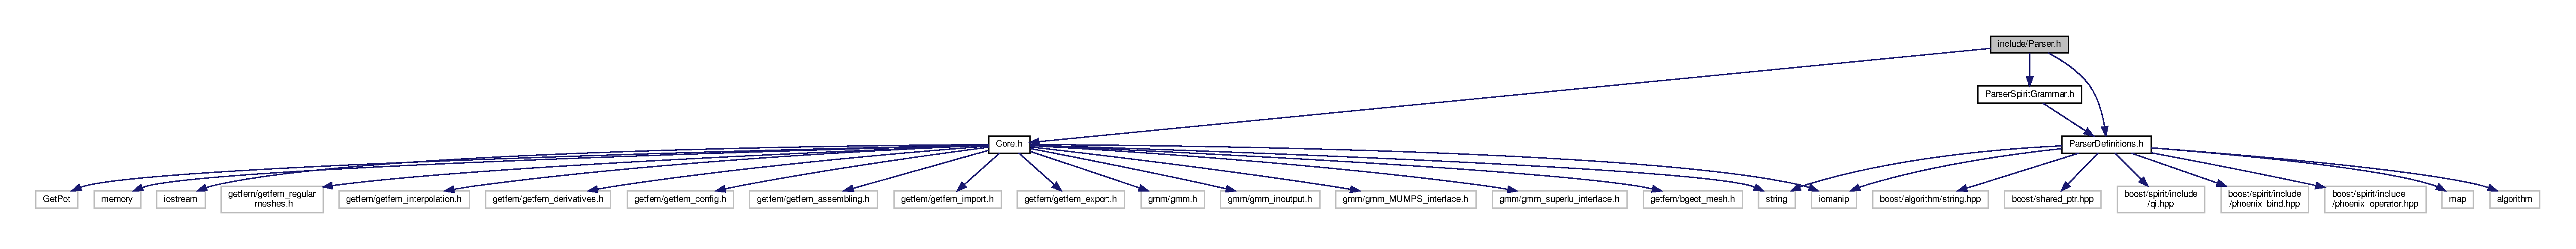
\includegraphics[width=350pt]{Parser_8h__incl}
\end{center}
\end{figure}
This graph shows which files directly or indirectly include this file\+:
\nopagebreak
\begin{figure}[H]
\begin{center}
\leavevmode
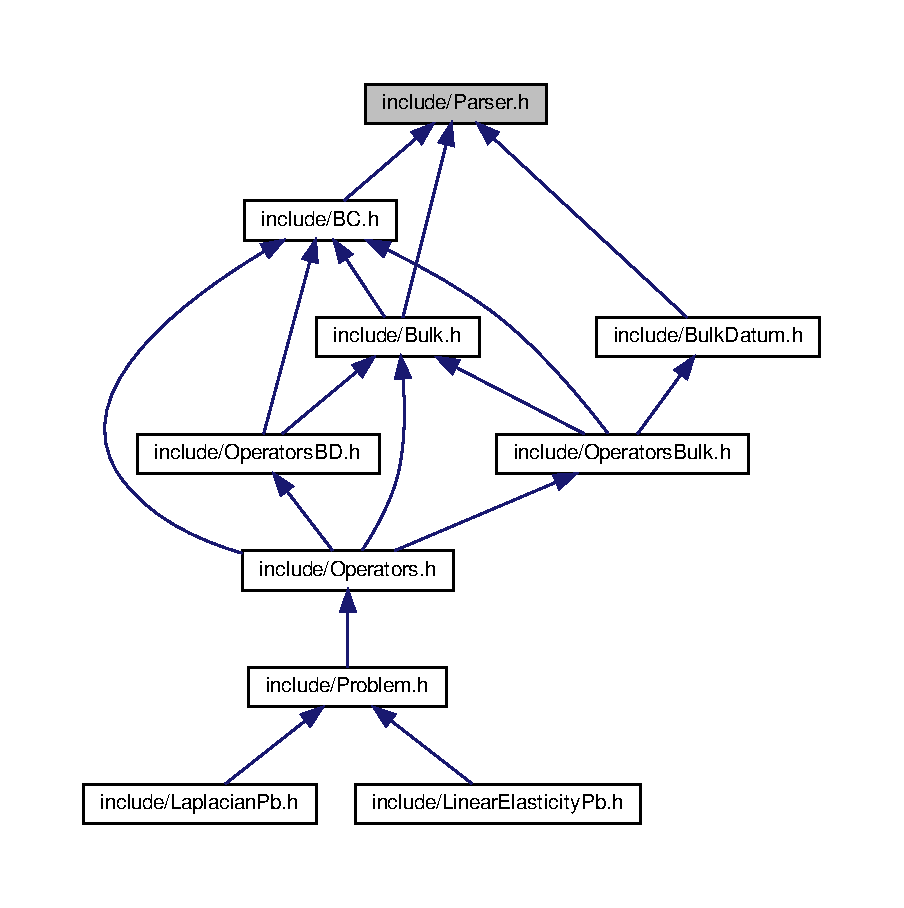
\includegraphics[width=350pt]{Parser_8h__dep__incl}
\end{center}
\end{figure}
\subsection*{Classes}
\begin{DoxyCompactItemize}
\item 
class \hyperlink{classLifeV_1_1Parser}{Life\+V\+::\+Parser}
\begin{DoxyCompactList}\small\item\em \hyperlink{classLifeV_1_1Parser}{Parser} -\/ A string parser for algebraic expressions. \end{DoxyCompactList}\end{DoxyCompactItemize}


\subsection{Detailed Description}
File containing the Parser interface. 

\begin{DoxyDate}{Date}
07-\/04-\/2009 
\end{DoxyDate}
\begin{DoxyAuthor}{Author}
Cristiano Malossi \href{mailto:cristiano.malossi@epfl.ch}{\tt cristiano.\+malossi@epfl.\+ch}
\end{DoxyAuthor}
Gilles Fourestey \href{mailto:gilles.fourestey@epfl.ch}{\tt gilles.\+fourestey@epfl.\+ch}  Cristiano Malossi \href{mailto:cristiano.malossi@epfl.ch}{\tt cristiano.\+malossi@epfl.\+ch} 
\hypertarget{ParserDefinitions_8h}{}\section{include/\+Parser\+Definitions.h File Reference}
\label{ParserDefinitions_8h}\index{include/\+Parser\+Definitions.\+h@{include/\+Parser\+Definitions.\+h}}


File containing the Parser definitions.  


{\ttfamily \#include $<$map$>$}\newline
{\ttfamily \#include $<$iomanip$>$}\newline
{\ttfamily \#include $<$string$>$}\newline
{\ttfamily \#include $<$algorithm$>$}\newline
{\ttfamily \#include $<$boost/algorithm/string.\+hpp$>$}\newline
{\ttfamily \#include $<$boost/shared\+\_\+ptr.\+hpp$>$}\newline
{\ttfamily \#include $<$boost/spirit/include/qi.\+hpp$>$}\newline
{\ttfamily \#include $<$boost/spirit/include/phoenix\+\_\+bind.\+hpp$>$}\newline
{\ttfamily \#include $<$boost/spirit/include/phoenix\+\_\+operator.\+hpp$>$}\newline
Include dependency graph for Parser\+Definitions.\+h\+:
\nopagebreak
\begin{figure}[H]
\begin{center}
\leavevmode
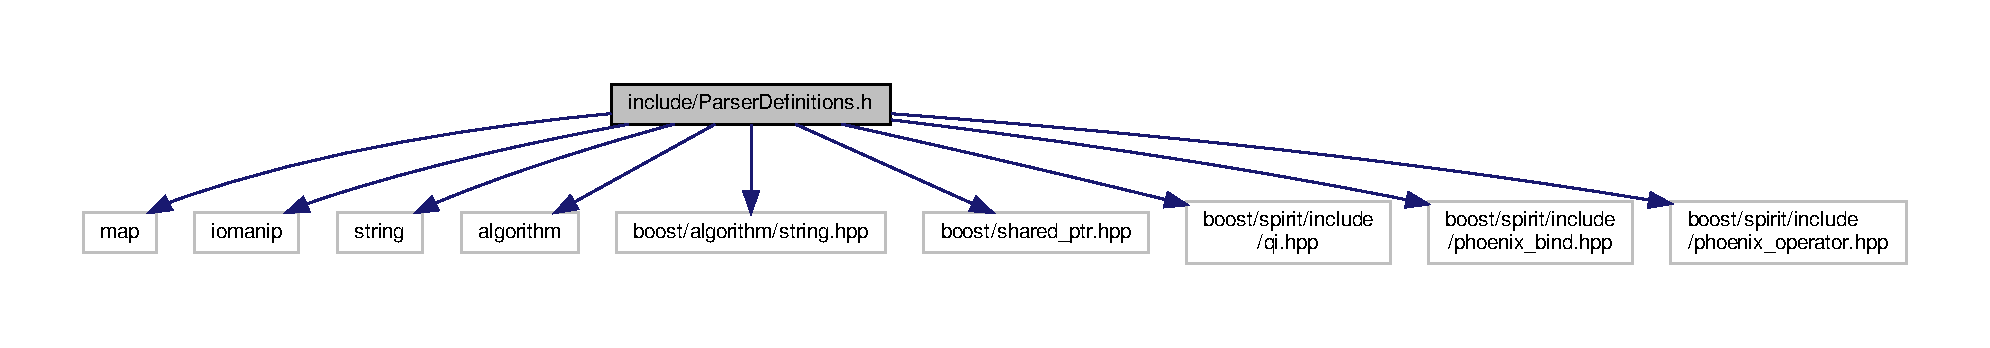
\includegraphics[width=350pt]{ParserDefinitions_8h__incl}
\end{center}
\end{figure}
This graph shows which files directly or indirectly include this file\+:
\nopagebreak
\begin{figure}[H]
\begin{center}
\leavevmode
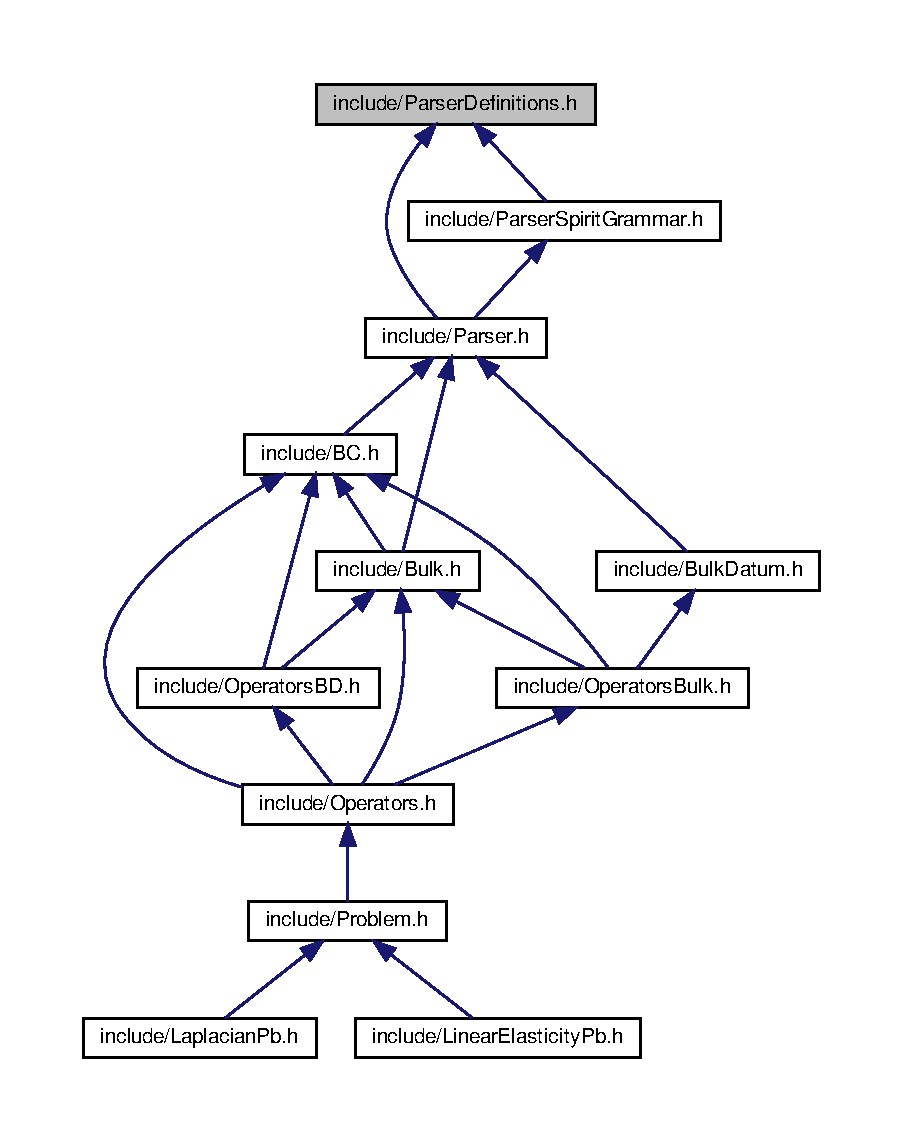
\includegraphics[width=350pt]{ParserDefinitions_8h__dep__incl}
\end{center}
\end{figure}


\subsection{Detailed Description}
File containing the Parser definitions. 

\begin{DoxyDate}{Date}
29-\/01-\/2010 
\end{DoxyDate}
\begin{DoxyAuthor}{Author}
Cristiano Malossi \href{mailto:cristiano.malossi@epfl.ch}{\tt cristiano.\+malossi@epfl.\+ch}
\end{DoxyAuthor}
Cristiano Malossi \href{mailto:cristiano.malossi@epfl.ch}{\tt cristiano.\+malossi@epfl.\+ch} 
\hypertarget{ParserSpiritGrammar_8h}{}\section{include/\+Parser\+Spirit\+Grammar.h File Reference}
\label{ParserSpiritGrammar_8h}\index{include/\+Parser\+Spirit\+Grammar.\+h@{include/\+Parser\+Spirit\+Grammar.\+h}}


File containing the Parser grammar.  


{\ttfamily \#include \char`\"{}Parser\+Definitions.\+h\char`\"{}}\newline
Include dependency graph for Parser\+Spirit\+Grammar.\+h\+:
\nopagebreak
\begin{figure}[H]
\begin{center}
\leavevmode
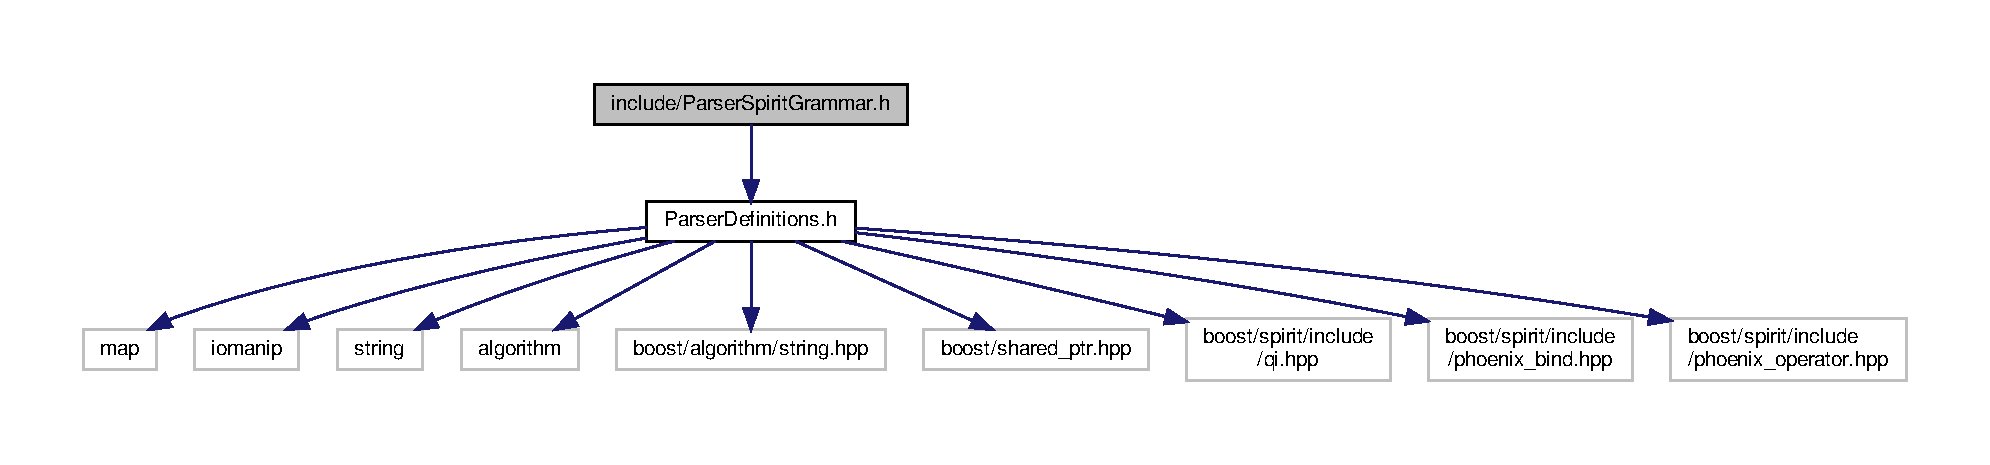
\includegraphics[width=350pt]{ParserSpiritGrammar_8h__incl}
\end{center}
\end{figure}
This graph shows which files directly or indirectly include this file\+:
\nopagebreak
\begin{figure}[H]
\begin{center}
\leavevmode
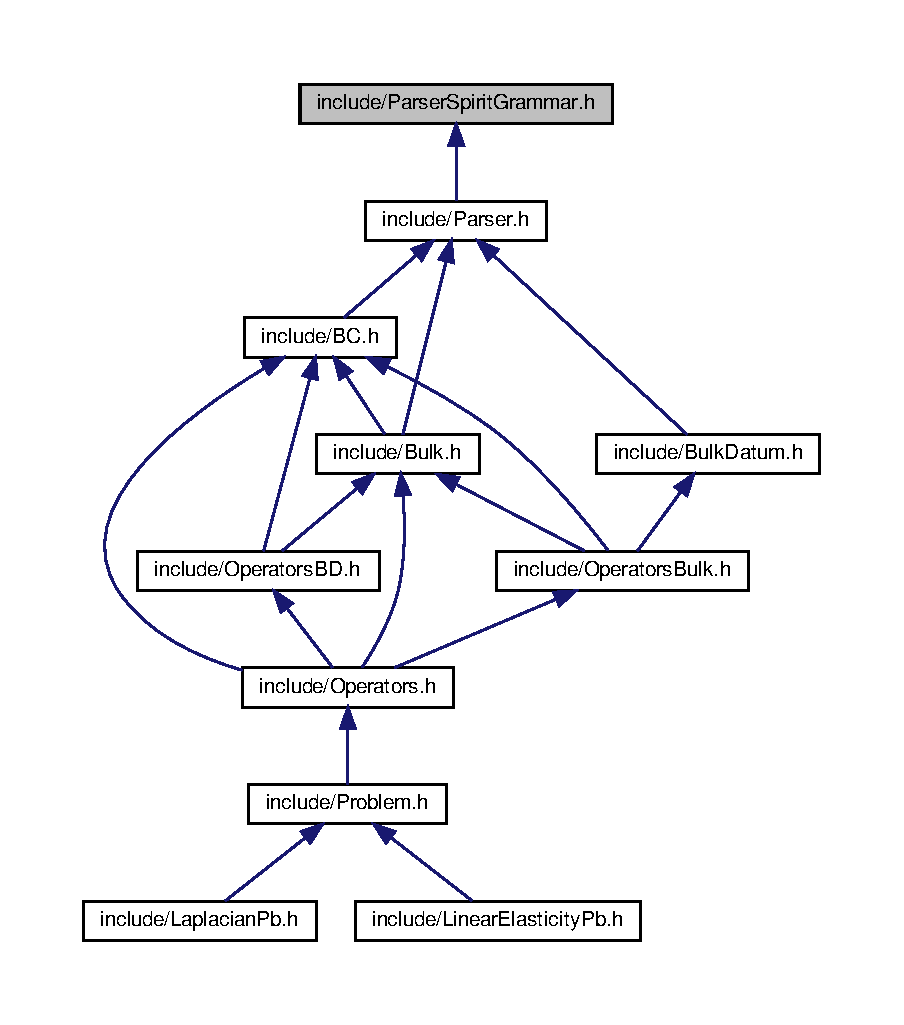
\includegraphics[width=350pt]{ParserSpiritGrammar_8h__dep__incl}
\end{center}
\end{figure}
\subsection*{Classes}
\begin{DoxyCompactItemize}
\item 
class \hyperlink{classLifeV_1_1ParserSpiritGrammar}{Life\+V\+::\+Parser\+Spirit\+Grammar$<$ Iterator\+Type, Results\+Type $>$}
\begin{DoxyCompactList}\small\item\em \hyperlink{classLifeV_1_1ParserSpiritGrammar}{Parser\+Spirit\+Grammar} -\/ A string parser grammar based on {\ttfamily boost\+::spirit\+::qi}. \end{DoxyCompactList}\end{DoxyCompactItemize}


\subsection{Detailed Description}
File containing the Parser grammar. 

\begin{DoxyDate}{Date}
05-\/02-\/2010 
\end{DoxyDate}
\begin{DoxyAuthor}{Author}
Cristiano Malossi \href{mailto:cristiano.malossi@epfl.ch}{\tt cristiano.\+malossi@epfl.\+ch}
\end{DoxyAuthor}
Cristiano Malossi \href{mailto:cristiano.malossi@epfl.ch}{\tt cristiano.\+malossi@epfl.\+ch} 
\hypertarget{StringUtility_8h}{}\doxysection{include/\+String\+Utility.h File Reference}
\label{StringUtility_8h}\index{include/StringUtility.h@{include/StringUtility.h}}


std\+::string utilities  


{\ttfamily \#include $<$cstdio$>$}\newline
{\ttfamily \#include $<$cstdlib$>$}\newline
{\ttfamily \#include $<$cstring$>$}\newline
{\ttfamily \#include $<$iosfwd$>$}\newline
{\ttfamily \#include $<$iostream$>$}\newline
{\ttfamily \#include $<$list$>$}\newline
{\ttfamily \#include $<$map$>$}\newline
{\ttfamily \#include $<$sstream$>$}\newline
{\ttfamily \#include $<$string$>$}\newline
{\ttfamily \#include $<$vector$>$}\newline
{\ttfamily \#include $<$boost/algorithm/string.\+hpp$>$}\newline
{\ttfamily \#include \char`\"{}Core.\+h\char`\"{}}\newline
Include dependency graph for String\+Utility.\+h\+:
% FIG 0
This graph shows which files directly or indirectly include this file\+:
% FIG 1
\doxysubsection*{Functions}
\begin{DoxyCompactItemize}
\item 
std\+::istream \& \mbox{\hyperlink{StringUtility_8h_a29b1aef17b4be5df580e406a5e140d62}{Life\+V\+::eat\+Line}} (std\+::istream \&s)
\item 
\mbox{\Hypertarget{StringUtility_8h_ae428ccb84b7baf4e4438e36a31f915d1}\label{StringUtility_8h_ae428ccb84b7baf4e4438e36a31f915d1}} 
std\+::istream \& \mbox{\hyperlink{StringUtility_8h_ae428ccb84b7baf4e4438e36a31f915d1}{Life\+V\+::eat\+Comments}} (std\+::istream \&s)
\begin{DoxyCompactList}\small\item\em skip lines starting with \textquotesingle{}!\%\#;\$\textquotesingle{} \end{DoxyCompactList}\item 
\mbox{\Hypertarget{StringUtility_8h_ae0b2f8ef96d797c86959535c8a5d81c2}\label{StringUtility_8h_ae0b2f8ef96d797c86959535c8a5d81c2}} 
std\+::istream \& \mbox{\hyperlink{StringUtility_8h_ae0b2f8ef96d797c86959535c8a5d81c2}{Life\+V\+::next\+Good\+Line}} (std\+::istream \&s, std\+::string \&line)
\begin{DoxyCompactList}\small\item\em gets next uncommented line \end{DoxyCompactList}\item 
std\+::string \& \mbox{\hyperlink{StringUtility_8h_aceb6f89371c24f4cddc8099ca7f91159}{Life\+V\+::set\+String\+Length}} (std\+::string \&s, unsigned int len, char c)
\item 
\mbox{\Hypertarget{StringUtility_8h_a1a787279805886c5b208055992c29c9a}\label{StringUtility_8h_a1a787279805886c5b208055992c29c9a}} 
int \mbox{\hyperlink{StringUtility_8h_a1a787279805886c5b208055992c29c9a}{Life\+V\+::atoi}} (const std\+::string \&s)
\begin{DoxyCompactList}\small\item\em extends atoi to S\+TL std\+::strings (from Stroustrup) \end{DoxyCompactList}\item 
\mbox{\Hypertarget{StringUtility_8h_af57500c586141320ace55cf0b2a5c9fe}\label{StringUtility_8h_af57500c586141320ace55cf0b2a5c9fe}} 
std\+::string {\bfseries Life\+V\+::operator+} (const std\+::string \&str, const int i)
\item 
\mbox{\Hypertarget{StringUtility_8h_ae00b5ce86e0f837f3f3392074652b7ed}\label{StringUtility_8h_ae00b5ce86e0f837f3f3392074652b7ed}} 
std\+::string {\bfseries Life\+V\+::operator+} (const std\+::string \&str, const long int i)
\item 
\mbox{\Hypertarget{StringUtility_8h_a54f5fa0ff0002920c744bcbaff350bc0}\label{StringUtility_8h_a54f5fa0ff0002920c744bcbaff350bc0}} 
std\+::string {\bfseries Life\+V\+::operator+} (const std\+::string \&str, const unsigned int i)
\item 
\mbox{\Hypertarget{StringUtility_8h_a200b22ebae8c113c2624f7195797d4a4}\label{StringUtility_8h_a200b22ebae8c113c2624f7195797d4a4}} 
{\footnotesize template$<$typename Entry\+Type $>$ }\\void {\bfseries Life\+V\+::parse\+List} (const std\+::string \&slist, std\+::list$<$ Entry\+Type $>$ \&list)
\item 
\mbox{\Hypertarget{StringUtility_8h_a95341022bde9111ea53dfe204cbe70ae}\label{StringUtility_8h_a95341022bde9111ea53dfe204cbe70ae}} 
double {\bfseries Life\+V\+::string2number} (const std\+::string \&s)
\item 
\mbox{\Hypertarget{StringUtility_8h_a3c2a31cefb08654a69273a1a3bf11fac}\label{StringUtility_8h_a3c2a31cefb08654a69273a1a3bf11fac}} 
{\footnotesize template$<$typename Number\+Type $>$ }\\std\+::string {\bfseries Life\+V\+::number2string} (const Number\+Type \&n)
\item 
\mbox{\Hypertarget{StringUtility_8h_a2e64a35012f78d9ab021477590e3bfaf}\label{StringUtility_8h_a2e64a35012f78d9ab021477590e3bfaf}} 
{\footnotesize template$<$typename Enumerator\+Type $>$ }\\std\+::string {\bfseries Life\+V\+::enum2\+String} (const Enumerator\+Type \&Enum, const std\+::map$<$ std\+::string, Enumerator\+Type $>$ \&Map)
\item 
\mbox{\Hypertarget{StringUtility_8h_a5f2c3319750ceebbeb2a3bb374a2596b}\label{StringUtility_8h_a5f2c3319750ceebbeb2a3bb374a2596b}} 
{\footnotesize template$<$typename Number\+Type $>$ }\\void {\bfseries Life\+V\+::string2numbers\+Vector} (const std\+::string \&string, std\+::vector$<$ Number\+Type $>$ \&number\+Vector)
\end{DoxyCompactItemize}


\doxysubsection{Detailed Description}
std\+::string utilities 

\begin{DoxyDate}{Date}
13-\/12-\/2010 
\end{DoxyDate}
\begin{DoxyAuthor}{Author}

\end{DoxyAuthor}
@maintainer Radu Popescu \href{mailto:radu.popescu@epfl.ch}{\texttt{ radu.\+popescu@epfl.\+ch}} 

\doxysubsection{Function Documentation}
\mbox{\Hypertarget{StringUtility_8h_a29b1aef17b4be5df580e406a5e140d62}\label{StringUtility_8h_a29b1aef17b4be5df580e406a5e140d62}} 
\index{StringUtility.h@{StringUtility.h}!eatLine@{eatLine}}
\index{eatLine@{eatLine}!StringUtility.h@{StringUtility.h}}
\doxysubsubsection{\texorpdfstring{eatLine()}{eatLine()}}
{\footnotesize\ttfamily std\+::istream\& Life\+V\+::eat\+Line (\begin{DoxyParamCaption}\item[{std\+::istream \&}]{s }\end{DoxyParamCaption})}

It gets a the next line from std\+::istream \mbox{\Hypertarget{StringUtility_8h_aceb6f89371c24f4cddc8099ca7f91159}\label{StringUtility_8h_aceb6f89371c24f4cddc8099ca7f91159}} 
\index{StringUtility.h@{StringUtility.h}!setStringLength@{setStringLength}}
\index{setStringLength@{setStringLength}!StringUtility.h@{StringUtility.h}}
\doxysubsubsection{\texorpdfstring{setStringLength()}{setStringLength()}}
{\footnotesize\ttfamily std\+::string\& Life\+V\+::set\+String\+Length (\begin{DoxyParamCaption}\item[{std\+::string \&}]{s,  }\item[{unsigned int}]{len,  }\item[{char}]{c }\end{DoxyParamCaption})}

always return a std\+::string with len characters
\begin{DoxyItemize}
\item if the s has more than len characters \+: keep only the first len
\item if the s has less than len characters \+: complete with c until len 
\end{DoxyItemize}
%--- End generated contents ---

% Index
\backmatter
\newpage
\phantomsection
\clearemptydoublepage
\addcontentsline{toc}{chapter}{Index}
\printindex

\end{document}
